% ─────────────────────────────────────────────────────────────────────────────
\chapter{Experimental Results and Operational Robustness Analysis}
\label{chap:results}
% ─────────────────────────────────────────────────────────────────────────────

This chapter presents the quantitative outcomes obtained from the
implementation documented in Chapter~\ref{chap:implementation} and interprets
them according to the methodological framework defined in
Chapter~\ref{chap:methodology}. The analysis focuses on the operational
robustness of \gls{ai}-based systems for automated image classification and
triage in forensic contexts.

A central feature of the evaluation is the parallel analysis of two
complementary system levels. The first comprises the transparent proxy models
defined in Section~\ref{subsec:implementation-architectures}, for which
predictions, maximum predicted-class probabilities, confusion matrices, and
internal attribution information are available. The second comprises the
selected black-box software systems, whose behavior is assessed exclusively
through observable and normalized outputs.

Both evaluation levels operate on the same frozen source population. The
1\,000 clean binary images and 500 clean \gls{ood} images constitute the common
source corpus, whereas 10\,000 adversarial and anti-forensic artifacts are
derived exclusively from the binary subset. The resulting comparison is
therefore based on the same underlying samples and experimental conditions,
while preserving the distinction between transparent model evaluation and
operational black-box assessment.

The purpose of the chapter is not to construct an absolute ranking among
heterogeneous systems or to reduce the study to a conventional
\gls{advml} benchmark. The systems differ in architecture, output semantics,
configuration, operational scope, and degree of transparency. Their results
are therefore interpreted from a forensic perspective, with particular
attention to false negatives on the firearm-oriented target category, false
positives on \texttt{non\_weapon} content, closed-set assignments of
\gls{ood} inputs, degradation under manipulated conditions, and the continued
need for human review
\cite{costantini2019digital,sanna2024preliminary,sanna2025pixelperfect}.

% ─────────────────────────────────────────────────────────────────────────────
\section{Experimental Evaluation Scope and Completeness}
\label{sec:results-scope}
% ─────────────────────────────────────────────────────────────────────────────

The experimental results cover the complete population generated through the
frozen implementation described in Chapter~\ref{chap:implementation}. The
common corpus contains 11\,500 logical experimental inputs, comprising clean
images and derived perturbed artifacts:

\begin{equation}
\begin{aligned}
N_{\mathrm{bundle}}
&=
1\,000\ \text{clean binary inputs}
+
500\ \text{\glsentryshort{ood} inputs}
\\
&\quad
+
5\,000\ \text{adversarial artifacts}
+
5\,000\ \text{anti-forensic artifacts}
\\
&=
11\,500.
\end{aligned}
\end{equation}

The proxy-model and black-box evaluations use different output
representations but cover the same experimental conditions. Each clean binary
input or perturbed binary artifact is evaluated by all three proxy
architectures through the checkpoint associated with its assigned fold.

The \gls{ood} branch follows a different proxy-model evaluation protocol. Each
of the 500 unique \gls{ood} images is evaluated by all five fold-specific
checkpoints of each architecture. The resulting 7\,500 prediction rows
therefore represent repeated checkpoint responses to 500 unique images and
must not be interpreted as 7\,500 independent \gls{ood} samples.

The black-box evaluation comprises four software families and six normalized
operational configurations. Magnet AXIOM/Magnet.AI, Griffeye/T3K CORE, and
Cellebrite Inseyets each contribute one configuration, whereas the D20, D50,
and D80 Excire Foto 2025 settings are retained as three separate
configurations. Each configuration produces one normalized decision for every
item in the 11\,500-file forensic evaluation bundle.

Table~\ref{tab:results-evaluation-completeness} summarizes the completeness of
the result population.

\begin{table}[H]
\centering
\small
\renewcommand{\arraystretch}{1.15}
\setlength{\tabcolsep}{5pt}
\caption{Completeness of the experimental result population}
\label{tab:results-evaluation-completeness}
\begin{tabularx}{0.96\textwidth}{@{}l r X@{}}
\toprule
\textbf{Result layer} &
\textbf{Records} &
\textbf{Coverage} \\
\midrule

Proxy-model predictions
&
40\,500
&
3\,000 clean predictions, 7\,500 fold-specific \gls{ood} responses, and
30\,000 predictions on adversarial and anti-forensic artifacts; no recorded
inference errors. \\

Normalized black-box decisions
&
69\,000
&
Six normalized configurations evaluated on all 11\,500 bundle items, with no
missing bundle-level decision. \\

Proxy binary-condition metrics
&
33
&
Three clean architecture-level rows and 30 architecture--perturbation
combinations. \\

Proxy robustness comparisons
&
30
&
Clean-to-perturbed comparisons for three architectures and ten perturbation
conditions. \\

Proxy \gls{ood} summaries
&
3
&
One fold-aggregated \gls{ood} record for each proxy architecture. \\

Black-box software metrics
&
186
&
Thirty-one aggregation records for each of the six normalized black-box
configurations. \\

Explainability cases
&
5
&
One representative case for each predefined diagnostic category, associated
with 20 thesis-level visual assets. \\

\bottomrule
\end{tabularx}
\end{table}

Binary accuracy, precision, recall, F1-score, \gls{fpr}, and \gls{fnr} are
computed exclusively on samples whose reference operational assignment is
\texttt{weapon} or \texttt{non\_weapon}. The \gls{ood} branch remains
separate and is analyzed through the proportion of inputs assigned to the
\texttt{weapon} class and, for the proxy models, through architecture-specific
maximum-probability indicators.

Accuracy drop, induced-error counts, directional error transitions, and the
confusion-matrix layout follow the definitions established in
Section~\ref{sec:methodology-evaluation-metrics}. Positive accuracy-drop values
indicate degradation relative to the clean baseline, whereas negative values
indicate a condition-specific increase in accuracy that must not be interpreted
as evidence of general robustness.

The clean-correct-to-incorrect transition rate is interpreted as attack success
rate only for the four model-dependent adversarial attacks: \gls{fgsm}, One
Pixel, Sigma-Zero, and SuperDeepFool. For Color Shift and the five
anti-forensic transformations, the same numerical transition is interpreted as
an induced-error rate rather than as adversarial or transfer success.

Maximum predicted-class probabilities are available only for the transparent
proxy models. They are retained as intra-model diagnostic indicators and are
not interpreted as calibrated probabilities directly comparable across
architectures. The selected black-box software systems do not expose
homogeneous numerical uncertainty measures; consequently, their comparison is
based on normalized observable decisions rather than cross-system confidence
scores.

% ─────────────────────────────────────────────────────────────────────────────
\section{Clean Baseline Performance}
\label{sec:results-clean-baseline}
% ─────────────────────────────────────────────────────────────────────────────

Evaluation on clean inputs establishes the nominal baseline against which
behavior under \gls{ood}, adversarial, and anti-forensic conditions is
subsequently assessed. The three proxy architectures were evaluated on the
frozen binary subset of 1\,000 images, comprising 500
\texttt{weapon} and 500 \texttt{non\_weapon} samples.

The positive class is \texttt{weapon}, and the negative class is
\texttt{non\_weapon}. A false negative therefore corresponds to a
\texttt{weapon} image classified as \texttt{non\_weapon}, whereas a false
positive corresponds to a \texttt{non\_weapon} image classified as
\texttt{weapon}.

Table~\ref{tab:results-clean-baseline-metrics} reports the principal clean
binary metrics. In addition to accuracy, balanced accuracy, macro-averaged
metrics, and class-specific performance for \texttt{weapon}, the table includes
the mean maximum predicted-class probability. This value is retained only as
an architecture-specific diagnostic of the output distribution and is not
interpreted as a calibrated confidence measure.

\begin{table}[H]
\centering
\scriptsize
\setlength{\tabcolsep}{2.3pt}
\renewcommand{\arraystretch}{1.15}
\caption{Clean performance of the proxy models on the binary subset}
\label{tab:results-clean-baseline-metrics}
\begin{tabularx}{\textwidth}{@{}l *{11}{>{\centering\arraybackslash}X}@{}}
\toprule
\textbf{Model} &
\textbf{Acc.} &
\textbf{Bal.} &
\textbf{M-P} &
\textbf{M-R} &
\textbf{M-F1} &
\textbf{P\textsubscript{w}} &
\textbf{R\textsubscript{w}} &
\textbf{F1\textsubscript{w}} &
\textbf{Max-P} &
\textbf{\acrshort{fpr}} &
\textbf{\acrshort{fnr}} \\
\midrule

EfficientNet-B0
& 0.978
& 0.978
& 0.978
& 0.978
& 0.978
& 0.972
& 0.984
& 0.978
& 0.979
& 0.028
& 0.016 \\

ResNet18
& 0.964
& 0.964
& 0.964
& 0.964
& 0.964
& 0.958
& 0.970
& 0.964
& 0.974
& 0.042
& 0.030 \\

\acrshort{clip}
& 0.927
& 0.927
& 0.933
& 0.927
& 0.927
& 0.881
& 0.988
& 0.931
& 0.559
& 0.134
& 0.012 \\

\bottomrule
\end{tabularx}

\vspace{0.4em}
\footnotesize
\textit{Note.} \textit{Bal.} indicates balanced accuracy; \textit{M-P},
\textit{M-R}, and \textit{M-F1} indicate macro-precision, macro-recall, and
macro-F1, respectively; \(P_w\), \(R_w\), and \(F1_w\) indicate precision,
recall, and F1-score for the \texttt{weapon} class. \textit{Max-P} indicates
the mean maximum predicted-class probability and is reported only as an
intra-model diagnostic indicator.
\end{table}

EfficientNet-B0 achieves the strongest overall clean-condition performance,
with an accuracy and macro-F1 of 0.978. Its \texttt{weapon} recall is 0.984,
corresponding to an \gls{fnr} of 0.016, while its \gls{fpr} is 0.028. Its mean
maximum predicted-class probability is 0.979.

ResNet18 shows slightly lower but still high clean-condition performance, with
an accuracy and macro-F1 of 0.964. Its \texttt{weapon} recall is 0.970, its
\gls{fnr} is 0.030, and its \gls{fpr} is 0.042. The corresponding mean maximum
predicted-class probability is 0.974.

The \gls{clip}-based proxy exhibits a different operational profile. Its
overall accuracy and macro-F1 are 0.927, lower than those of the two
fully fine-tuned \glspl{cnn}. However, it achieves the highest
\texttt{weapon} recall, at 0.988, and the lowest \gls{fnr}, at 0.012. This
reduction in missed \texttt{weapon} samples is accompanied by an
\gls{fpr} of 0.134, substantially higher than those of EfficientNet-B0 and
ResNet18.

The mean maximum predicted-class probability of the \gls{clip}-based proxy is
0.559. This value must not be compared directly with the corresponding values
of the convolutional architectures because the probability outputs are not
calibrated across models. Within the \gls{clip}-based proxy, it indicates that
the strong tendency to assign inputs to the \texttt{weapon} class does not
generally coincide with maximum probabilities close to one.

This behavior is not the result of zero-shot classification. In the adopted
implementation, \gls{clip} serves as a pretrained and frozen visual encoder
connected to a supervised binary classification head trained on the same
frozen binary task. Its error profile must therefore be attributed to the
combination of the pretrained visual representation and the learned binary
decision head rather than to the original image--text similarity interface.

Table~\ref{tab:results-clean-confusion-matrices} reports the aggregate
confusion-matrix components for the three proxy models. The layout is:

\[
\mathbf{C}
=
\begin{bmatrix}
\glsentryshort{tn} & \glsentryshort{fp} \\
\glsentryshort{fn} & \glsentryshort{tp}
\end{bmatrix}.
\]

\begin{table}[H]
\centering
\caption{Clean confusion matrices of the proxy models}
\label{tab:results-clean-confusion-matrices}
\begin{tabular}{@{}l r r r r@{}}
\toprule
\textbf{Model} &
\textbf{\gls{tn}} &
\textbf{\gls{fp}} &
\textbf{\gls{fn}} &
\textbf{\gls{tp}} \\
\midrule

EfficientNet-B0
& 486
& 14
& 8
& 492 \\

ResNet18
& 479
& 21
& 15
& 485 \\

\gls{clip}
& 433
& 67
& 6
& 494 \\

\bottomrule
\end{tabular}
\end{table}

The same error distributions are visualized in
Figure~\ref{fig:results-clean-confusion-matrices}. EfficientNet-B0 minimizes
the total number of errors, producing 22 incorrect decisions. ResNet18 produces
36 errors and maintains an intermediate profile. The \gls{clip}-based proxy
produces 73 errors, but only six of them are false negatives; the remaining 67
are false positives.

\begin{figure}[htbp]
\centering

\begin{minipage}{0.48\textwidth}
\centering
\small EfficientNet-B0

\vspace{0.2em}
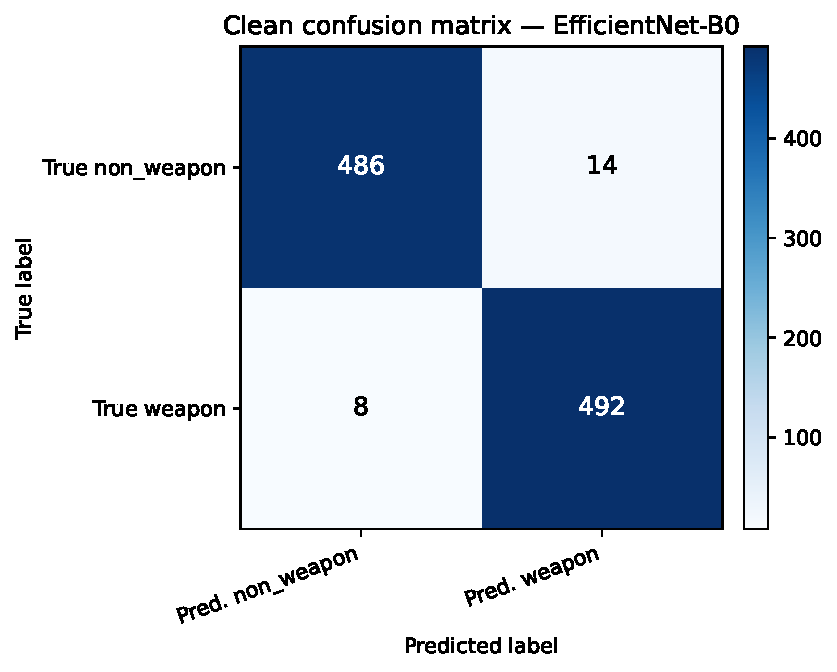
\includegraphics[width=\linewidth]
{images/fig_clean_confusion_matrix_efficientnet_b0.pdf}
\end{minipage}
\hfill
\begin{minipage}{0.48\textwidth}
\centering
\small ResNet18

\vspace{0.2em}
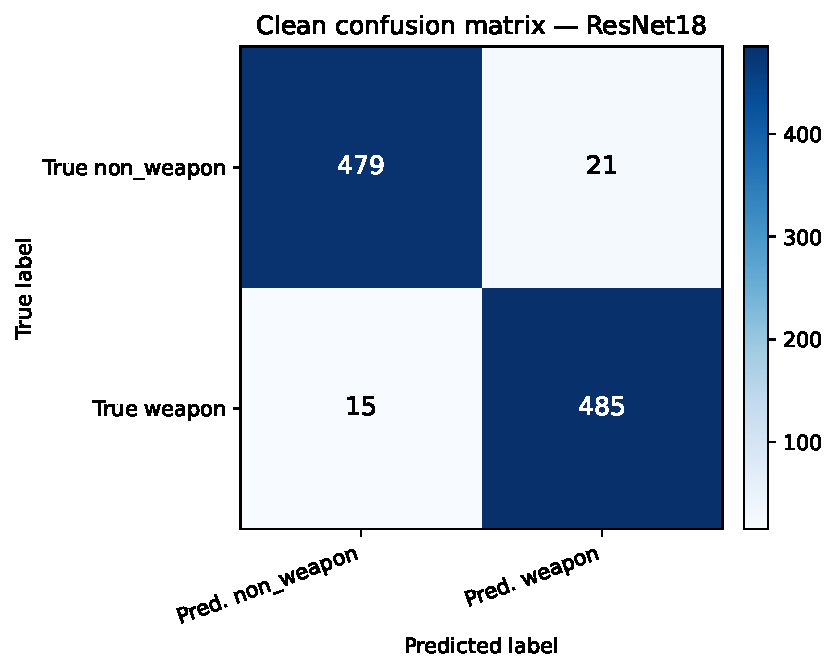
\includegraphics[width=\linewidth]
{images/fig_clean_confusion_matrix_resnet18.pdf}
\end{minipage}

\vspace{0.8em}

\begin{minipage}{0.58\textwidth}
\centering
\small \acrshort{clip}

\vspace{0.2em}
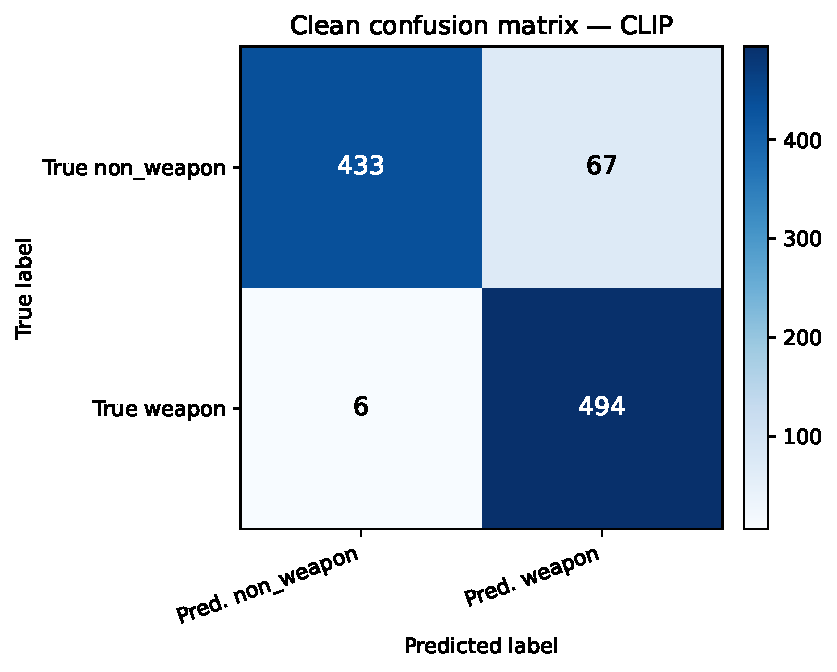
\includegraphics[width=\linewidth]
{images/fig_clean_confusion_matrix_clip.pdf}
\end{minipage}

\caption{Clean confusion matrices of the three proxy models on the binary
subset}
\label{fig:results-clean-confusion-matrices}
\end{figure}

From a forensic-triage perspective, the most consequential distinction concerns
the direction of the errors. EfficientNet-B0 provides the strongest overall
balance, with eight false negatives and 14 false positives. ResNet18 produces
15 false negatives and 21 false positives. The \gls{clip}-based proxy reduces
false negatives to six but increases false positives to 67.

The clean comparison therefore cannot be interpreted solely through aggregate
accuracy. A lower false-negative rate may reduce the risk of failing to flag
firearm-oriented content, but a higher false-positive rate increases the volume
of irrelevant material presented for human review. Conversely, minimizing the
review workload must not be achieved by accepting an operationally
unacceptable number of missed target images.

Overall, all three proxy architectures achieve high performance under clean
conditions, but they expose distinct operational tradeoffs among target-class
recall, false-negative risk, false-positive workload, and model-specific output
distributions. These differences provide the necessary baseline for evaluating
whether the same profiles remain stable under \gls{ood}, adversarial, and
anti-forensic conditions.

% ─────────────────────────────────────────────────────────────────────────────
\section{\texorpdfstring{\gls{ood}}{Out-of-Distribution} Behavior}
\label{sec:results-ood}
% ─────────────────────────────────────────────────────────────────────────────

The \gls{ood} evaluation examines the behavior of the three proxy architectures
on the separate 500-image \gls{ood} branch. As established in
Chapter~\ref{chap:methodology}, these images are not treated as a third
supervised class and do not contribute to binary accuracy, precision, recall,
or confusion-matrix counts.

The analysis instead characterizes how inputs outside the frozen binary
distribution are forced into one of the two available closed-set operational
classes
\cite{hendrycks2017baseline,liang2018odin,fort2021exploring}.

Each of the 500 unique \gls{ood} images was evaluated by all five
fold-specific checkpoints of each proxy architecture:

\begin{equation}
500\ \text{unique \glsentryshort{ood} images}
\times
5\ \text{fold-specific checkpoints}
=
2\,500\ \text{responses per architecture}.
\end{equation}

The resulting responses are not independent images. They represent five
fold-specific model outputs for each unique \gls{ood} input. The reported
counts and rates therefore characterize checkpoint-response behavior rather
than unique-image-level classification frequency.

Two principal indicators are considered:

\begin{itemize}
\item the \emph{weapon assignment rate}, defined as the proportion of the
2\,500 responses assigned to \texttt{weapon};

\item the \emph{high-maximum-probability rate}, defined as the proportion of
responses whose maximum predicted-class probability is at least 0.90.
\end{itemize}

Neither indicator represents supervised correctness because the \gls{ood}
inputs have no binary reference assignment.

Table~\ref{tab:results-ood-behavior} reports the fold-aggregated results.

\begin{table}[H]
\centering
\scriptsize
\setlength{\tabcolsep}{3.5pt}
\renewcommand{\arraystretch}{1.15}
\caption{Fold-aggregated behavior of the proxy models on \gls{ood} inputs}
\label{tab:results-ood-behavior}
\begin{tabular}{@{}l r r r r r r r@{}}
\toprule
\textbf{Model} &
\textbf{Responses} &
\textbf{\shortstack{Weapon\\responses}} &
\textbf{\shortstack{Non-weapon\\responses}} &
\textbf{W-rate} &
\textbf{Max-P} &
\textbf{HP-count} &
\textbf{HP-rate} \\
\midrule

EfficientNet-B0
& 2\,500
& 924
& 1\,576
& 0.3696
& 0.8505
& 1\,252
& 0.5008 \\

ResNet18
& 2\,500
& 1\,094
& 1\,406
& 0.4376
& 0.8896
& 1\,617
& 0.6468 \\

\acrshort{clip}
& 2\,500
& 2\,089
& 411
& 0.8356
& 0.5358
& 0
& 0.0000 \\

\bottomrule
\end{tabular}

\vspace{0.4em}
\footnotesize
\textit{Note.} \textit{W-rate} indicates the proportion of fold-specific
responses assigned to \texttt{weapon}; \textit{Max-P} indicates the mean
maximum predicted-class probability; \textit{HP-count} indicates the number of
responses whose maximum probability is at least 0.90; and \textit{HP-rate}
indicates the corresponding proportion over the 2\,500 responses. Each total
comprises five checkpoint responses for each of the 500 unique \gls{ood}
images.
\end{table}

The \gls{clip}-based proxy exhibits the strongest tendency to assign
\gls{ood} inputs to the firearm-oriented class. It produces 2\,089
\texttt{weapon} responses, corresponding to a weapon assignment rate of
0.8356. However, its mean maximum predicted-class probability is only 0.5358,
and none of its 2\,500 responses reaches the threshold of 0.90.

The zero high-maximum-probability rate must therefore not be interpreted as an
absence of \texttt{weapon} assignments. Instead, the \gls{clip}-based proxy
frequently selects \texttt{weapon} while producing output probabilities close
to the central region of the binary output range. This combination indicates a
strong directional assignment tendency without high maximum-probability
responses under the adopted threshold.

EfficientNet-B0 and ResNet18 assign lower proportions of the \gls{ood}
responses to \texttt{weapon}. EfficientNet-B0 produces 924 such responses,
corresponding to a rate of 0.3696, whereas ResNet18 produces 1\,094, for a rate
of 0.4376.

Their model-specific output distributions nevertheless contain substantially
more responses above the 0.90 threshold. EfficientNet-B0 produces 1\,252
high-maximum-probability responses, corresponding to a rate of 0.5008.
ResNet18 produces 1\,617, corresponding to the highest rate among the three
architectures, at 0.6468.

Figure~\ref{fig:results-ood-weapon-rate-confidence} compares the weapon
assignment rate, mean maximum predicted-class probability, and
high-maximum-probability rate.

\begin{figure}[H]
\centering
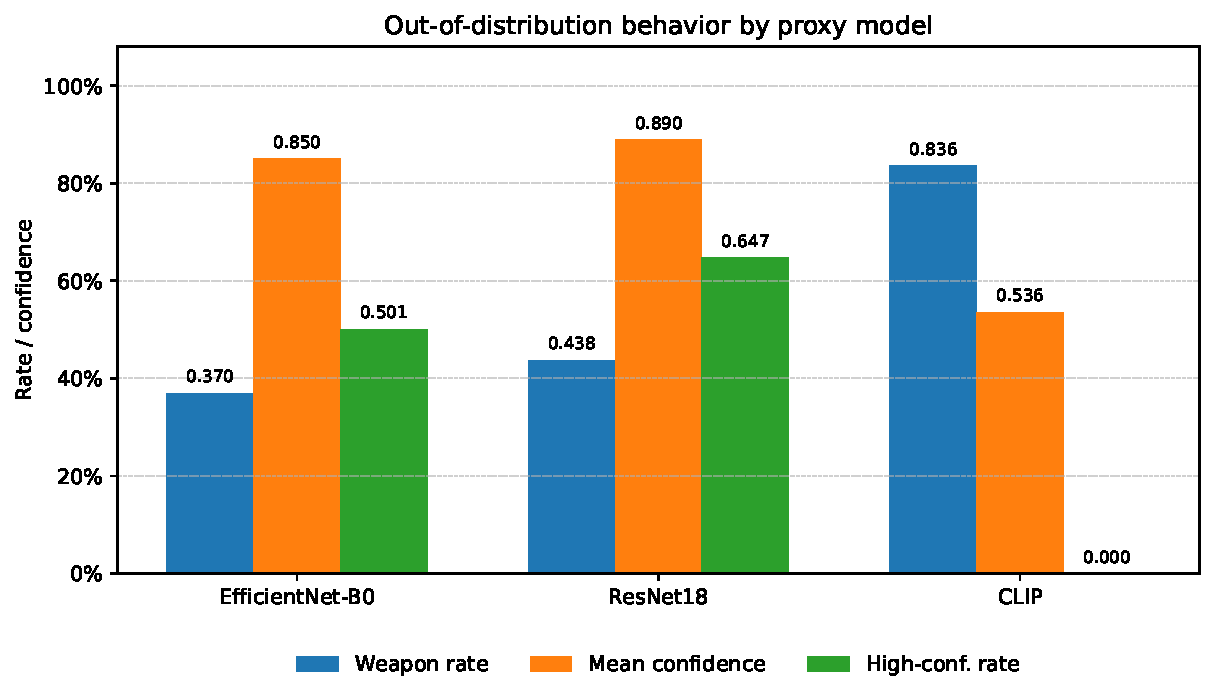
\includegraphics[width=0.95\textwidth]
{images/fig_ood_weapon_rate_and_confidence.pdf}
\caption{Weapon assignment rate and maximum predicted-class probability
indicators on \gls{ood} inputs}
\label{fig:results-ood-weapon-rate-confidence}
\end{figure}

The figure highlights that weapon assignment frequency and maximum-probability
behavior represent distinct dimensions of the closed-set response. The
\gls{clip}-based proxy exhibits the highest weapon assignment rate but the
lowest mean maximum probability and no responses above the 0.90 threshold.
ResNet18 exhibits the highest high-maximum-probability rate despite assigning
fewer responses to \texttt{weapon}. EfficientNet-B0 presents an intermediate
profile for both indicators.

These values are architecture-specific and must not be used to construct a
cross-model probability or uncertainty ranking. The output probabilities were
not calibrated across architectures, and the same numerical value may not
represent the same degree of uncertainty for EfficientNet-B0, ResNet18, and the
\gls{clip}-based proxy.

Figure~\ref{fig:results-ood-confidence-distribution} presents the complete
distribution of maximum predicted-class probabilities for the three
architectures.

\begin{figure}[H]
\centering
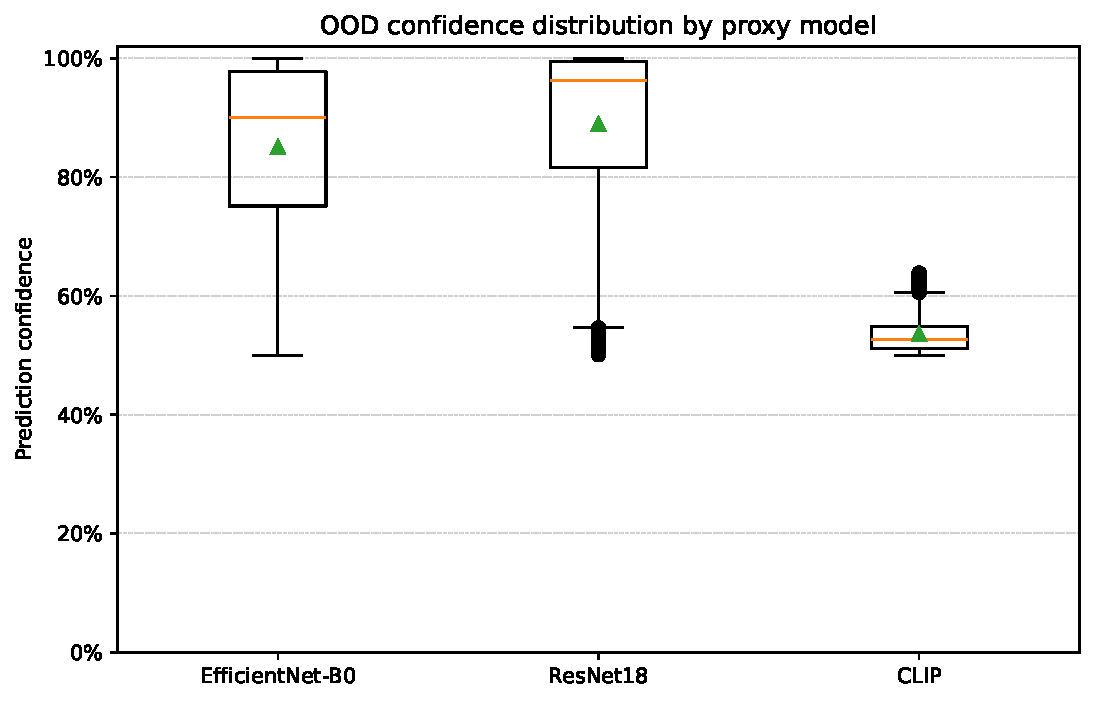
\includegraphics[width=0.95\textwidth]
{images/fig_ood_confidence_distribution.pdf}
\caption{Distribution of maximum predicted-class probabilities on
\gls{ood} inputs for each proxy architecture}
\label{fig:results-ood-confidence-distribution}
\end{figure}

The distributional view confirms that the responses of the \gls{clip}-based
proxy remain below the predefined 0.90 threshold, whereas EfficientNet-B0 and
ResNet18 produce substantial populations above it. This difference does not
establish that one architecture is intrinsically more reliable on
out-of-distribution content. It characterizes the architecture-specific score
profiles produced when all inputs must be assigned to one of two closed-set
classes.

From a forensic perspective, a \texttt{weapon} assignment on the \gls{ood}
branch is not a false positive in the supervised binary sense. The input has no
\texttt{weapon} or \texttt{non\_weapon} reference assignment. Nevertheless,
such an output may still affect triage by increasing the quantity of unrelated
material prioritized for review.

Conversely, a high maximum predicted-class probability on an \gls{ood} input
does not demonstrate that the assignment is semantically valid. It indicates
only that the corresponding proxy architecture produced a strongly peaked
closed-set output for material outside the frozen binary evaluation
distribution.

The \gls{ood} results therefore identify two operationally relevant but
separate behaviors:

\begin{itemize}
\item the tendency to route distributionally different material toward the
firearm-oriented review category;

\item the tendency to produce high maximum predicted-class probabilities for
forced closed-set assignments.
\end{itemize}

Both behaviors can influence prioritization and analyst workload. Neither can
be treated as stand-alone evidence, supervised correctness, or calibrated
uncertainty, and both remain subject to human verification
\cite{guo2017calibration,nist2023airmf}.

% ─────────────────────────────────────────────────────────────────────────────
\section{Anti-Forensic Robustness}
\label{sec:results-antiforensic}
% ─────────────────────────────────────────────────────────────────────────────

The anti-forensic evaluation examines the stability of the proxy models under
five deterministic, model-agnostic image transformations. These conditions do
not require access to model parameters, gradients, logits, or decision
thresholds. They represent operations compatible with ordinary image
circulation and processing, although the same transformations may also be
applied intentionally to alter observable image characteristics
\cite{stamm2010anti,yaacoub2021digital,hendrycks2019benchmarking}.

The evaluated conditions comprise JPEG recompression, downsampling followed by
resizing to the original dimensions, Gaussian blurring, histogram
modification, and contrast stretching. Their operational relevance derives
from the fact that they may occur during compression, platform-mediated
sharing, editing, conversion, or deliberate anti-forensic manipulation.

For each architecture and transformation, performance is compared with the
corresponding clean baseline. Accuracy drop is defined as:

\begin{equation}
\Delta_{\mathrm{acc}}
=
\mathrm{Acc}_{\mathrm{clean}}
-
\mathrm{Acc}_{\mathrm{transformed}}.
\end{equation}

Positive values indicate lower aggregate accuracy under the transformed
condition. A value of zero indicates unchanged aggregate accuracy, whereas a
negative value indicates higher accuracy on the specific transformed
population.

A zero or negative accuracy drop must not be interpreted as evidence that the
transformation introduced no adverse decisions. Aggregate accuracy may remain
unchanged or increase when some clean-condition errors are corrected while
other initially correct samples become incorrect. For this reason, accuracy
drop is examined together with the induced-error count, induced-error rate, and
direction of the clean-correct-to-incorrect transitions.

Table~\ref{tab:results-antiforensic-robustness} reports transformed accuracy and
accuracy drop for all architecture--transformation combinations.

\begin{table}[H]
\centering
\scriptsize
\setlength{\tabcolsep}{3.3pt}
\renewcommand{\arraystretch}{1.15}
\caption{Accuracy and accuracy drop under anti-forensic transformations}
\label{tab:results-antiforensic-robustness}
\begin{tabular}{@{}l r r r r r r@{}}
\toprule
\textbf{Transformation} &
\textbf{\gls{clip} acc.} &
\textbf{Drop} &
\textbf{EffNet acc.} &
\textbf{Drop} &
\textbf{ResNet acc.} &
\textbf{Drop} \\
\midrule

\gls{jpegrecompression}
& 0.925
& 0.002
& 0.976
& 0.002
& 0.964
& 0.000 \\

\gls{resampleresize}
& 0.929
& -0.002
& 0.976
& 0.002
& 0.963
& 0.001 \\

\gls{gaussianblur}
& 0.934
& -0.007
& 0.965
& 0.013
& 0.959
& 0.005 \\

\gls{histogrammodification}
& 0.925
& 0.002
& 0.973
& 0.005
& 0.934
& 0.030 \\

\gls{contraststretching}
& 0.927
& 0.000
& 0.974
& 0.004
& 0.963
& 0.001 \\

\bottomrule
\end{tabular}

\vspace{0.4em}
\footnotesize
\textit{Note.} Drop is computed as clean accuracy minus transformed accuracy.
Positive values indicate aggregate degradation, zero indicates unchanged
aggregate accuracy, and negative values indicate a condition-specific increase.
None of these values alone establishes the absence or presence of newly induced
errors.
\end{table}

Figure~\ref{fig:results-antiforensic-accuracy-drop-heatmap} presents the same
comparison as a heatmap.

\begin{figure}[H]
\centering
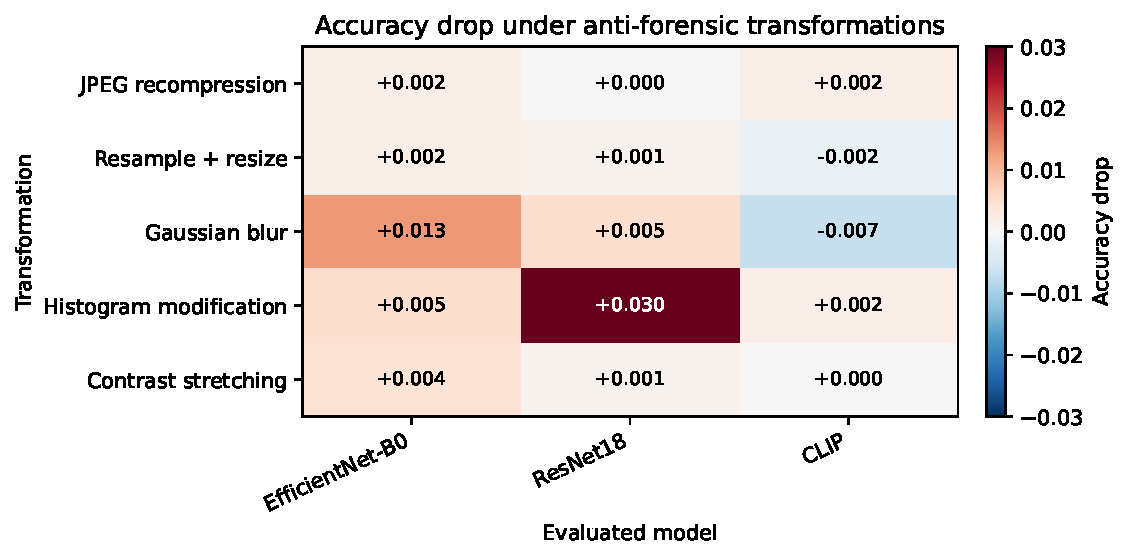
\includegraphics[width=0.88\textwidth]
{images/fig_anti_forensic_accuracy_drop_heatmap.pdf}
\caption{Accuracy drop of the proxy models under anti-forensic transformations}
\label{fig:results-antiforensic-accuracy-drop-heatmap}
\end{figure}

The aggregate results indicate that the five transformations produce smaller
accuracy variations than the strongest model-dependent adversarial attacks
examined in Section~\ref{sec:results-adversarial}. This relative difference
does not make the anti-forensic effects operationally negligible. Even limited
aggregate degradation may correspond to newly missed target-category images.

EfficientNet-B0 remains above 0.965 accuracy under every transformation.
Gaussian Blur produces its largest degradation, reducing accuracy from 0.978
to 0.965 and yielding an accuracy drop of 0.013. Histogram Modification is the
second most influential condition for this model, with an accuracy of 0.973 and
a drop of 0.005.

ResNet18 is most affected by Histogram Modification. Its accuracy decreases
from 0.964 to 0.934, corresponding to the largest anti-forensic accuracy drop
observed across the three architectures, at 0.030. Gaussian Blur produces a
smaller reduction to 0.959, corresponding to a drop of 0.005. JPEG
Recompression leaves aggregate accuracy unchanged at 0.964.

The \gls{clip}-based proxy exhibits small aggregate variations across the five
conditions. JPEG Recompression and Histogram Modification reduce accuracy by
0.002, Contrast Stretching leaves it unchanged, and Resample Resize increases
it by 0.002. Gaussian Blur increases aggregate accuracy from 0.927 to 0.934.

These limited or negative accuracy drops must be interpreted cautiously. They
do not demonstrate that the \gls{clip}-based proxy is unaffected by the
transformations. A transformed population can contain both newly introduced
errors and corrected clean-condition errors, with the latter compensating for
the former in the aggregate accuracy.

Table~\ref{tab:results-antiforensic-operational-errors} reports the most
operationally relevant condition for each architecture. The selected conditions
capture the largest aggregate degradation or, where aggregate drops are tied or
limited, the greatest newly induced error burden.

\begin{table}[H]
\centering
\scriptsize
\setlength{\tabcolsep}{3.5pt}
\renewcommand{\arraystretch}{1.15}
\caption{Operational indicators for representative anti-forensic conditions}
\label{tab:results-antiforensic-operational-errors}
\begin{tabular}{@{}l l r r r r r@{}}
\toprule
\textbf{Model} &
\textbf{Transformation} &
\textbf{Induced} &
\textbf{IER} &
\textbf{Max-P shift} &
\textbf{W\(\rightarrow\)NW} &
\textbf{NW\(\rightarrow\)W} \\
\midrule

EfficientNet-B0
& \gls{gaussianblur}
& 17
& 0.0174
& -0.0099
& 17
& 0 \\

ResNet18
& \gls{histogrammodification}
& 39
& 0.0405
& -0.0157
& 23
& 16 \\

\acrshort{clip}
& \gls{histogrammodification}
& 13
& 0.0140
& -0.0037
& 6
& 7 \\

\bottomrule
\end{tabular}

\vspace{0.4em}
\footnotesize
\textit{Note.} \textit{Induced} is the number of clean-correct samples rendered
incorrect by the transformation. \textit{IER} is the induced-error rate over
the clean-correct denominator. \textit{Max-P shift} is the mean transformed
maximum predicted-class probability minus the corresponding clean value.
W\(\rightarrow\)NW denotes \texttt{weapon}-to-\texttt{non\_weapon}
transitions; NW\(\rightarrow\)W denotes the opposite direction.
\end{table}

For EfficientNet-B0, Gaussian Blur introduces 17 errors among samples that were
correctly classified in their clean form. All 17 transitions occur from
\texttt{weapon} to \texttt{non\_weapon}, producing an induced-error rate of
0.0174. The direction of these transitions is operationally more consequential
than the aggregate drop alone because every newly induced error corresponds to
a missed firearm-oriented sample.

For ResNet18, Histogram Modification introduces 39 errors and produces the
highest anti-forensic induced-error rate, at 0.0405. Of these transitions, 23
occur from \texttt{weapon} to \texttt{non\_weapon}, while 16 occur from
\texttt{non\_weapon} to \texttt{weapon}. The condition therefore increases
both missed-target risk and false-positive review workload.

For the \gls{clip}-based proxy, Histogram Modification introduces 13 errors
among clean-correct samples, corresponding to an induced-error rate of 0.0140.
Six transitions occur from \texttt{weapon} to \texttt{non\_weapon}, and seven
occur in the opposite direction. Although the aggregate accuracy drop is only
0.002, the transition analysis confirms that the transformed condition is not
behaviorally identical to the clean baseline.

The maximum-probability shifts for the three representative cases are negative,
but their magnitudes are limited. These values indicate a reduction in the
mean maximum predicted-class probability relative to the corresponding clean
predictions. They do not constitute calibrated uncertainty estimates and
cannot be compared directly across architectures.

The results also demonstrate why aggregate accuracy and induced-error rate
must remain separate. For example, Gaussian Blur increases the aggregate
accuracy of the \gls{clip}-based proxy by 0.007 while still inducing four new
errors among clean-correct samples. The aggregate improvement therefore
reflects the net balance between newly introduced errors and previously
incorrect decisions that become correct, rather than the absence of
transformation sensitivity.

From an operational perspective, the anti-forensic results identify
architecture- and transformation-specific failure modes rather than a uniform
degradation pattern. Gaussian Blur primarily affects EfficientNet-B0 through
new \texttt{weapon}-to-\texttt{non\_weapon} transitions, whereas Histogram
Modification produces the largest effects for ResNet18 and the most relevant
transition burden for the \gls{clip}-based proxy.

These findings are important because the evaluated transformations do not
require model access and may arise during routine handling, conversion,
compression, editing, or re-sharing. In a forensic workflow, even modest
aggregate variation may become consequential when it produces missed
target-category images, increases irrelevant review volume, or interacts with
low visual quality and ambiguous context.

The anti-forensic evaluation therefore does not support a general claim that
the proxy architectures are robust to ordinary image transformations. It shows
that their aggregate accuracy is comparatively stable under the frozen
conditions, while also revealing specific clean-correct samples whose
operational assignments change. These outputs remain triage indicators and
must be subject to systematic human verification.

% ─────────────────────────────────────────────────────────────────────────────
\section{Adversarial Robustness}
\label{sec:results-adversarial}
% ─────────────────────────────────────────────────────────────────────────────

The adversarial evaluation examines the response of the transparent proxy
models to perturbations generated to alter classifier behavior
\cite{szegedy2014intriguing,goodfellow2015explaining,biggio2018wild}. These
conditions are used to assess operational robustness in a controlled forensic
evaluation rather than to construct an independent \gls{advml} benchmark.

Four model-dependent attacks were generated against the fold-specific
EfficientNet-B0 checkpoints. \gls{fgsm}, \gls{sigmazero}, and
\gls{superdeepfool} used white-box checkpoint access, whereas
\gls{onepixel} used score-based access to the same target architecture.
Evaluation of these artifacts on EfficientNet-B0 constitutes direct-target
assessment.

The same artifacts were subsequently evaluated on ResNet18 and the
\gls{clip}-based proxy to measure empirical transfer behavior. Their effects on
these architectures must therefore not be interpreted as white-box attacks
against ResNet18 or \gls{clip}
\cite{biggio2018wild,nowroozi2021survey,barni2018cf}.

\gls{colorshift} is treated separately as a deterministic, model-agnostic
adversarial-style condition. It does not use model parameters, gradients,
scores, or checkpoints and is therefore not associated with a target-model
attack success rate.

For every architecture and condition, accuracy drop is defined as:

\begin{equation}
\Delta_{\mathrm{acc}}
=
\mathrm{Acc}_{\mathrm{clean}}
-
\mathrm{Acc}_{\mathrm{perturbed}}.
\end{equation}

Positive values indicate lower aggregate accuracy under the perturbed
condition. Zero indicates unchanged aggregate accuracy, whereas negative
values indicate a condition-specific increase.

As in the anti-forensic analysis, zero or negative accuracy drop does not imply
that no new errors were introduced. Newly incorrect decisions may be offset by
clean-condition errors that become correct under the perturbed distribution.

For the four model-dependent attacks, attack success rate is computed over the
clean-correct population:

\begin{equation}
\mathrm{ASR}
=
\frac{
N\!\left(
\widehat{y}_{\mathrm{clean}}=y
\land
\widehat{y}_{\mathrm{perturbed}}\neq y
\right)
}{
N\!\left(
\widehat{y}_{\mathrm{clean}}=y
\right)
}.
\end{equation}

This definition differs from the generation-time success indicator recorded
while creating the artifacts. The results reported here use matched clean and
perturbed predictions and exclude samples already misclassified in their clean
form from the ASR denominator.

Table~\ref{tab:results-adversarial-robustness} reports perturbed accuracy and
accuracy drop for the five evaluated conditions.

\begin{table}[H]
\centering
\scriptsize
\setlength{\tabcolsep}{3.3pt}
\renewcommand{\arraystretch}{1.15}
\caption{Accuracy and accuracy drop under adversarial and adversarial-style
conditions}
\label{tab:results-adversarial-robustness}
\begin{tabular}{@{}l r r r r r r@{}}
\toprule
\textbf{Condition} &
\textbf{\gls{clip} acc.} &
\textbf{Drop} &
\textbf{EffNet acc.} &
\textbf{Drop} &
\textbf{ResNet acc.} &
\textbf{Drop} \\
\midrule

\gls{fgsm}
& 0.914
& 0.013
& 0.575
& 0.403
& 0.918
& 0.046 \\

\gls{superdeepfool}
& 0.926
& 0.001
& 0.931
& 0.047
& 0.964
& 0.000 \\

\gls{sigmazero}
& 0.944
& -0.017
& 0.015
& 0.963
& 0.968
& -0.004 \\

\gls{onepixel}
& 0.928
& -0.001
& 0.976
& 0.002
& 0.963
& 0.001 \\

\gls{colorshift}
& 0.925
& 0.002
& 0.977
& 0.001
& 0.963
& 0.001 \\

\bottomrule
\end{tabular}

\vspace{0.4em}
\footnotesize
\textit{Note.} The first four conditions were generated against fold-specific
EfficientNet-B0 checkpoints. Their evaluation on ResNet18 and the
\acrshort{clip}-based proxy measures transfer behavior. Color Shift is
model-agnostic. Drop is computed as clean accuracy minus perturbed accuracy;
negative values indicate a condition-specific aggregate increase and do not
establish the absence of newly induced errors.
\end{table}

Figure~\ref{fig:results-adversarial-accuracy-drop-heatmap} visualizes the
accuracy-drop distribution. The concentration of the largest values in the
EfficientNet-B0 column reflects the fact that the four model-dependent attacks
were generated against this architecture.

\begin{figure}[H]
\centering
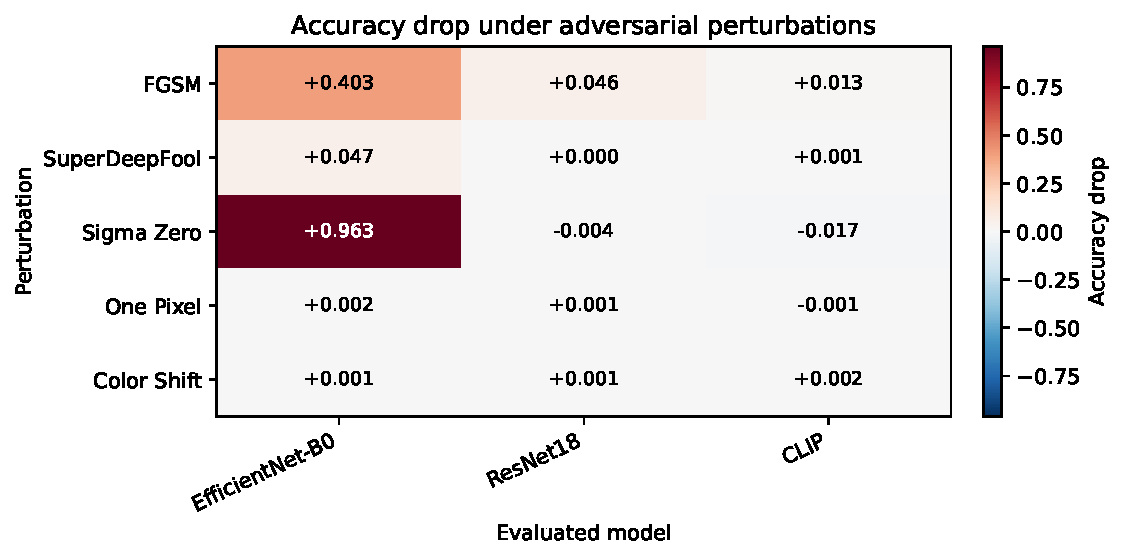
\includegraphics[width=0.88\textwidth]
{images/fig_adversarial_accuracy_drop_heatmap.pdf}
\caption{Accuracy drop of the proxy models under adversarial and
adversarial-style conditions}
\label{fig:results-adversarial-accuracy-drop-heatmap}
\end{figure}

The most severe result is observed for EfficientNet-B0 under
\gls{sigmazero}. Accuracy decreases from 0.978 to 0.015, corresponding to a
drop of 0.963. Among the 978 samples classified correctly in their clean form,
963 become incorrect, yielding an ASR of 0.9847.

The directional transitions are nearly balanced: 489 clean-correct
\texttt{weapon} samples become \texttt{non\_weapon}, while 474
clean-correct \texttt{non\_weapon} samples become \texttt{weapon}. The result
therefore represents a near-total collapse of the direct-target classifier
rather than a degradation confined to one class.

The operational consequence is twofold. The 489
\texttt{weapon}-to-\texttt{non\_weapon} transitions correspond to newly
missed firearm-oriented images, while the 474 transitions in the opposite
direction substantially increase irrelevant review workload.

\gls{fgsm} also produces severe direct-target degradation. EfficientNet-B0
accuracy decreases to 0.575, corresponding to a drop of 0.403. The attack
induces 406 errors among clean-correct samples and reaches an ASR of 0.4151.

In this case, the directional distribution is strongly asymmetric. Of the 406
induced errors, 321 are \texttt{weapon}-to-\texttt{non\_weapon}
transitions, whereas 85 occur in the opposite direction. FGSM therefore
produces a particularly relevant missed-target risk in addition to its
aggregate performance degradation.

\gls{superdeepfool} has a smaller direct-target effect. EfficientNet-B0
accuracy decreases to 0.931, producing a drop of 0.047 and an ASR of 0.0481.
All 47 induced errors occur from \texttt{non\_weapon} to \texttt{weapon};
no clean-correct \texttt{weapon} image becomes \texttt{non\_weapon} under
this condition.

This distinction is operationally important. The aggregate accuracy drop
indicates reduced correctness, but the observed direct-target failure mode
increases false-positive review workload without introducing additional missed
firearm-oriented images among the clean-correct target samples.

\gls{onepixel} produces only two direct-target induced errors on
EfficientNet-B0, one in each direction, corresponding to an ASR of 0.0020.
Its perturbed accuracy is 0.976, only 0.002 below the clean baseline. Under the
frozen parameters, this score-based condition is therefore substantially less
effective against the target architecture than Sigma-Zero, FGSM, or
SuperDeepFool.

Table~\ref{tab:results-adversarial-operational-errors} summarizes the most
relevant direct-target and transferred model-dependent conditions.

\begin{table}[H]
\centering
\scriptsize
\setlength{\tabcolsep}{3.5pt}
\renewcommand{\arraystretch}{1.15}
\caption{Operational indicators for selected model-dependent adversarial
conditions}
\label{tab:results-adversarial-operational-errors}
\begin{tabular}{@{}l l r r r r r@{}}
\toprule
\textbf{Model} &
\textbf{Attack} &
\textbf{Induced} &
\textbf{ASR} &
\textbf{Max-P shift} &
\textbf{W\(\rightarrow\)NW} &
\textbf{NW\(\rightarrow\)W} \\
\midrule

EfficientNet-B0
& \gls{sigmazero}
& 963
& 0.9847
& -0.2578
& 489
& 474 \\

EfficientNet-B0
& \gls{fgsm}
& 406
& 0.4151
& -0.1246
& 321
& 85 \\

EfficientNet-B0
& \gls{superdeepfool}
& 47
& 0.0481
& -0.3063
& 0
& 47 \\

ResNet18
& \gls{fgsm}
& 47
& 0.0488
& -0.0230
& 27
& 20 \\

\acrshort{clip}
& \gls{fgsm}
& 23
& 0.0248
& -0.0043
& 8
& 15 \\

\bottomrule
\end{tabular}

\vspace{0.4em}
\footnotesize
\textit{Note.} \textit{Induced} is the number of clean-correct samples rendered
incorrect by the perturbed condition. \textit{ASR} uses the clean-correct
denominator. \textit{Max-P shift} is the mean perturbed maximum
predicted-class probability minus the corresponding clean value.
W\(\rightarrow\)NW denotes \texttt{weapon}-to-\texttt{non\_weapon}
transitions; NW\(\rightarrow\)W denotes the opposite direction.
\end{table}

The maximum-probability shift must be interpreted independently of the
direction and number of induced errors. For example, SuperDeepFool produces the
largest negative shift among the selected EfficientNet-B0 conditions, at
\(-0.3063\), but induces substantially fewer errors than Sigma-Zero or FGSM.
Moreover, all of its induced errors occur in the false-positive direction.

The shift is computed from the maximum predicted-class probability before and
after perturbation. The maximizing class may differ between the clean and
perturbed predictions. Consequently, the value does not measure the probability
change of a fixed class and does not constitute a calibrated uncertainty
estimate.

The transfer assessment shows that perturbations optimized against
EfficientNet-B0 do not produce equivalent effects on the other proxy
architectures. The largest transferred degradation occurs under FGSM.
ResNet18 accuracy decreases from 0.964 to 0.918, corresponding to a drop of
0.046, 47 induced errors, and an ASR of 0.0488. Twenty-seven of these errors are
\texttt{weapon}-to-\texttt{non\_weapon} transitions.

For the \gls{clip}-based proxy, FGSM decreases accuracy from 0.927 to 0.914,
corresponding to a drop of 0.013. It induces 23 errors and reaches an ASR of
0.0248. Eight transitions occur from \texttt{weapon} to
\texttt{non\_weapon}, while 15 occur in the opposite direction.

Transferred Sigma-Zero artifacts do not reproduce the direct-target collapse.
ResNet18 accuracy increases by 0.004 and the \gls{clip}-based proxy accuracy
increases by 0.017. These aggregate increases nevertheless coexist with three
induced errors for ResNet18 and eight for \gls{clip}. The result again confirms
that aggregate improvement does not establish sample-level invariance.

Transferred SuperDeepFool and One Pixel artifacts produce limited effects.
SuperDeepFool induces no errors among clean-correct ResNet18 samples and three
among clean-correct \gls{clip} samples. One Pixel induces one error for
ResNet18 and none for \gls{clip} under the frozen evaluation.

Color Shift produces only marginal aggregate changes across the three
architectures. Because it is model-agnostic, its clean-correct-to-incorrect
transitions are interpreted as induced errors rather than attack or transfer
success. Its role is to provide a common adversarial-style comparison condition
rather than evidence of white-box vulnerability.

The adversarial results therefore identify a strong dependence on the
relationship between the perturbation-generation model and the evaluated
architecture. EfficientNet-B0 achieves the highest clean accuracy but undergoes
the most severe degradation when the attacks are optimized directly against
its fold-specific checkpoints. The same artifacts transfer only partially to
ResNet18 and the \gls{clip}-based proxy.

This limited transferability must not be interpreted as general robustness of
the non-target architectures. It establishes only that the frozen
EfficientNet-B0-oriented perturbations were less effective against the other
proxy models. A direct attack generated against ResNet18 or the
\gls{clip}-based proxy could produce a different result and was outside the
experimental scope.

From a forensic perspective, the findings demonstrate that high clean accuracy
does not ensure operational stability under deliberately manipulated inputs.
They also show that aggregate degradation alone is insufficient: the same
accuracy drop may represent newly missed target images, increased false-positive
workload, or a combination of both.

The output of an \gls{ai}-based classification model must therefore remain a
triage indicator rather than autonomous evidence. Its use requires systematic
human verification, traceable processing, explicit knowledge of the evaluated
threat model, and awareness that robustness conclusions are bounded to the
tested architectures, perturbations, parameters, and access assumptions.

% ─────────────────────────────────────────────────────────────────────────────
\section{Black-Box Software Results}
\label{sec:results-commercial}
% ─────────────────────────────────────────────────────────────────────────────

The implementation-specific configurations, observable output fields,
operational mappings, and normalization procedures adopted for the selected
black-box software systems are documented in
Section~\ref{sec:implementation-forensic-tools}. The present section reports
the resulting normalized behavior without making assumptions about inaccessible
internal architectures, training data, thresholds, or confidence-calibration
procedures.

The analysis comprises four software families and six normalized operational
configurations:

\begin{itemize}
\item \gls{magnetaxiomtool}/\gls{magnetai};
\item \gls{griffeye}/\gls{t3kcore};
\item \gls{excirefoto2025} under the \texttt{D20}, \texttt{D50}, and
\texttt{D80} semantic-distance settings;
\item \gls{cellebriteinseyets}.
\end{itemize}

Each configuration produced one normalized decision for every item in the
11\,500-file forensic evaluation bundle. The complete black-box population
therefore contains:

\begin{equation}
6\ \text{normalized configurations}
\times
11\,500\ \text{bundle items}
=
69\,000\ \text{matched decisions}.
\end{equation}

No bundle item remained without a matched normalized decision, and the
canonical public population contains no \texttt{unknown} outputs. Non-bundle
records present in some controlled raw exports were excluded during
normalization, as described in
Section~\ref{subsec:implementation-normalization}.

The 11\,500 matched decisions associated with each configuration comprise two
analytically distinct populations:

\begin{itemize}
\item 11\,000 binary items with a reference operational assignment of
\texttt{weapon} or \texttt{non\_weapon};

\item 500 \gls{ood} inputs, analyzed separately through their observable
weapon assignment rate.
\end{itemize}

Accuracy, balanced accuracy, precision, recall, \gls{fnr}, and \gls{fpr} are
computed only on the 11\,000 interpretable binary items. The \gls{ood} inputs
are excluded from those metrics because they have no binary reference
assignment.

The binary aggregate is itself bundle-weighted rather than
condition-balanced. It contains 1\,000 clean inputs and 10\,000 perturbed
artifacts:

\begin{equation}
N_{\mathrm{binary}}
=
1\,000\ \text{clean inputs}
+
5\,000\ \text{adversarial artifacts}
+
5\,000\ \text{anti-forensic artifacts}
=
11\,000.
\end{equation}

Consequently, the bundle-level metrics are influenced primarily by behavior on
the perturbed population. They must not be interpreted as the arithmetic mean
of clean, adversarial, and anti-forensic performance, nor as estimates of the
frequency with which these conditions would occur in an operational case.

The four model-dependent adversarial conditions were generated against
fold-specific EfficientNet-B0 checkpoints. Their evaluation through the
selected black-box software systems therefore constitutes an empirical transfer
assessment. It does not constitute a white-box attack against any commercial
system. \gls{colorshift} instead provides a deterministic model-agnostic
comparison condition.

Table~\ref{tab:results-commercial-overview} summarizes the normalized results
for the six configurations.

\begin{table}[H]
\centering
\scriptsize
\renewcommand{\arraystretch}{1.15}
\setlength{\tabcolsep}{2.6pt}
\caption{Bundle-weighted summary of the selected black-box software
configurations}
\label{tab:results-commercial-overview}
\resizebox{\textwidth}{!}{%
\begin{tabular}{@{}l r r r r r r r r@{}}
\toprule
\textbf{Configuration} &
\textbf{Matched} &
\textbf{Clean \acrshort{fnr}} &
\textbf{Bundle Acc.} &
\textbf{Bundle Bal.} &
\textbf{Bundle R\textsubscript{w}} &
\textbf{Bundle \acrshort{fnr}} &
\textbf{Bundle \acrshort{fpr}} &
\textbf{\acrshort{ood} W-rate} \\
\midrule

\gls{magnetaxiomtool}/\gls{magnetai}
& 11\,500
& 0.070
& 0.933
& 0.933
& 0.901
& 0.099
& 0.035
& 0.360 \\

\gls{griffeye}/\gls{t3kcore}
& 11\,500
& 0.036
& 0.972
& 0.972
& 0.951
& 0.049
& 0.007
& 0.260 \\

\gls{excirefoto2025} \texttt{D20}
& 11\,500
& 0.120
& 0.911
& 0.911
& 0.857
& 0.143
& 0.036
& 0.238 \\

\gls{excirefoto2025} \texttt{D50}
& 11\,500
& 0.042
& 0.925
& 0.925
& 0.949
& 0.051
& 0.099
& 0.340 \\

\gls{excirefoto2025} \texttt{D80}
& 11\,500
& 0.014
& 0.887
& 0.887
& 0.981
& 0.019
& 0.207
& 0.522 \\

\gls{cellebriteinseyets}
& 11\,500
& 0.032
& 0.958
& 0.958
& 0.958
& 0.042
& 0.042
& 0.292 \\

\bottomrule
\end{tabular}%
}

\vspace{0.4em}
\footnotesize
\textit{Note.} \textit{Matched} indicates the complete 11\,500-item bundle
population associated with each normalized configuration. Clean
\acrshort{fnr} is computed on the 1\,000 unperturbed binary inputs. Bundle
accuracy, balanced accuracy, weapon recall, \acrshort{fnr}, and \acrshort{fpr}
are computed on the 11\,000-item binary population, comprising clean,
adversarial, and anti-forensic samples and excluding \gls{ood} inputs.
\textit{\acrshort{ood} W-rate} indicates the proportion of the 500
\gls{ood} inputs assigned to \texttt{weapon}. The bundle-level values reflect
the frozen experimental composition and do not constitute general validation
or an absolute ranking of the selected software systems.
\end{table}

Figure~\ref{fig:results-forensic-tools-global-comparison} visualizes the same
bundle-weighted metrics.

\begin{figure}[H]
\centering
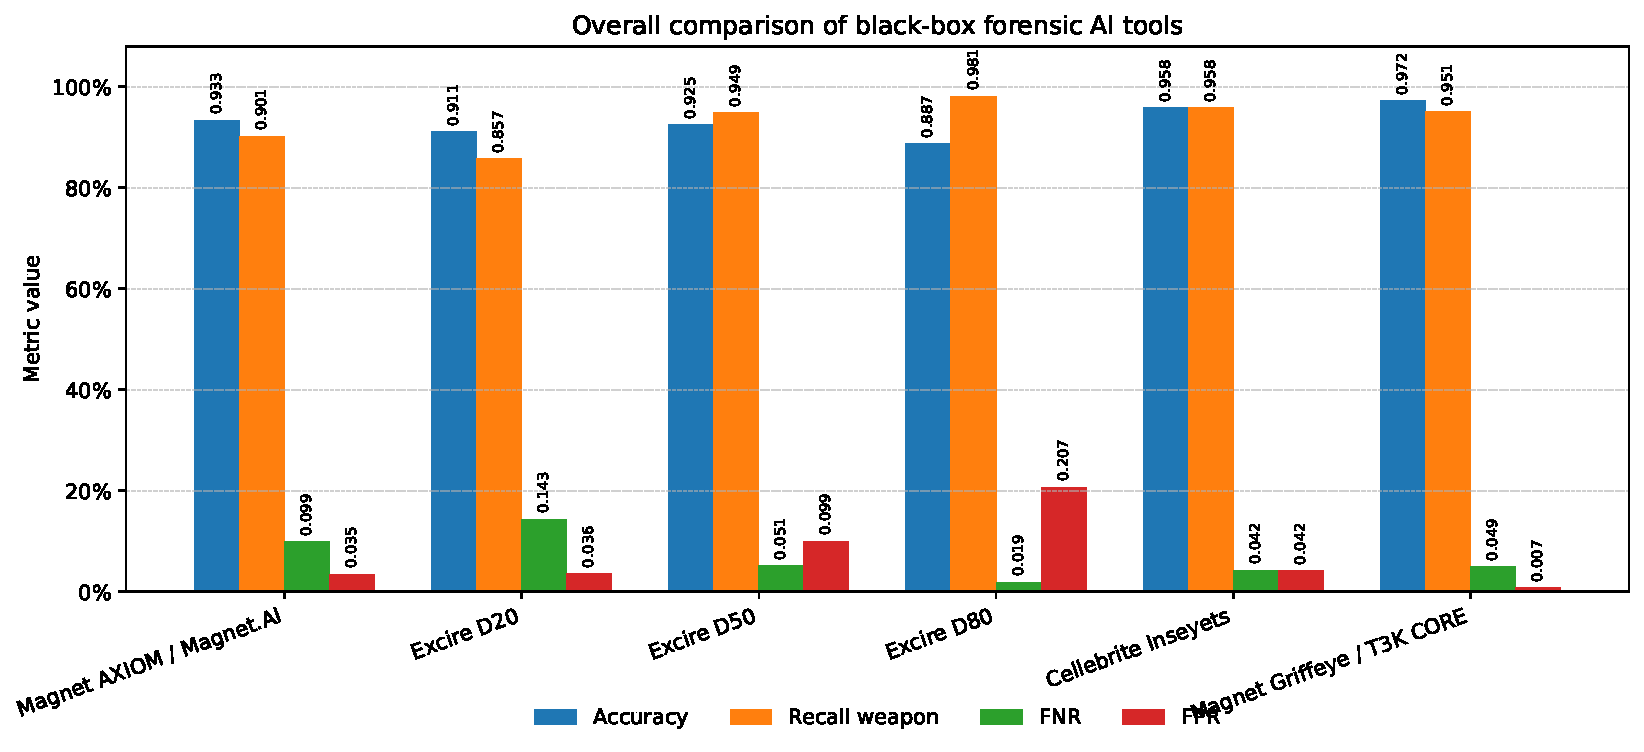
\includegraphics[width=\textwidth]
{images/fig_forensic_tools_global_metrics_comparison.pdf}
\caption{Bundle-weighted normalized metrics of the selected black-box software
configurations}
\label{fig:results-forensic-tools-global-comparison}
\end{figure}

The aggregate comparison identifies distinct operational profiles, but it must
not be interpreted as a direct ranking of intrinsic system quality. The
evaluated software systems differ in intended use, internal taxonomy,
observable output semantics, configuration, and decision mechanism.
Furthermore, the binary bundle contains repeated manipulated versions derived
from the same 1\,000 source images rather than 11\,000 independent real-world
cases.

Within the frozen protocol, \gls{griffeye}/\gls{t3kcore} exhibits the highest
bundle-level accuracy, at 0.972, and the lowest \gls{fpr}, at 0.007. Its
weapon recall is 0.951, corresponding to a bundle \gls{fnr} of 0.049.

\gls{cellebriteinseyets} presents a comparatively balanced profile. Its bundle
accuracy is 0.958, weapon recall is 0.958, \gls{fnr} is 0.042, and
\gls{fpr} is 0.042.

\gls{magnetaxiomtool}/\gls{magnetai} achieves a bundle accuracy of 0.933 and
an \gls{fpr} of 0.035. Its weapon recall is lower, at 0.901, corresponding to
a bundle \gls{fnr} of 0.099. Its clean \gls{fnr}, at 0.070, is lower than the
bundle-weighted value, indicating a larger missed-target proportion across the
combined perturbed population.

The three \gls{excirefoto2025} configurations expose the clearest
configuration-dependent tradeoff. At \texttt{D20}, the system produces a
relatively low \gls{fpr} of 0.036 and the lowest \gls{ood} weapon assignment
rate, at 0.238, but its weapon recall is 0.857 and its \gls{fnr} is 0.143.

At \texttt{D50}, weapon recall increases to 0.949 and the \gls{fnr} decreases
to 0.051. This improvement is accompanied by an \gls{fpr} of 0.099 and an
\gls{ood} weapon assignment rate of 0.340.

At \texttt{D80}, weapon recall reaches 0.981 and the \gls{fnr} decreases to
0.019, the lowest among the six configurations. However, the \gls{fpr}
increases to 0.207, and the \gls{ood} weapon assignment rate reaches 0.522.
The broader retrieval setting therefore minimizes missed firearm-oriented
content at the cost of a substantially larger false-positive review burden.

The Excire results demonstrate why a configuration with lower \gls{fnr} is not
automatically preferable in every operational context. Increasing retrieval
coverage can reduce missed detections while simultaneously increasing the
quantity of \texttt{non\_weapon} and \gls{ood} material routed to the
firearm-oriented review category.

Figure~\ref{fig:results-forensic-tools-ood-weapon-flag-rate} reports the
observable weapon assignment rate on the separate \gls{ood} branch.

\begin{figure}[H]
\centering
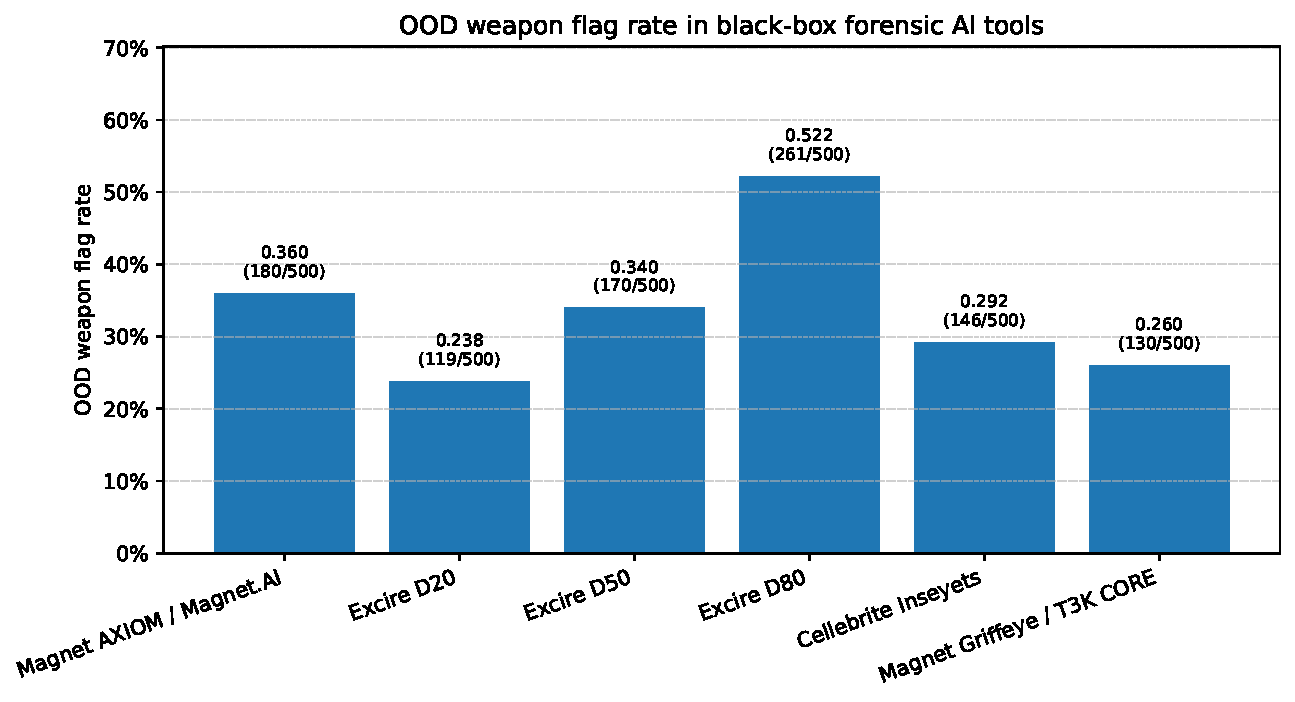
\includegraphics[width=0.90\textwidth]
{images/fig_forensic_tools_ood_weapon_flag_rate.pdf}
\caption{Weapon assignment rate of the selected black-box software
configurations on \gls{ood} inputs}
\label{fig:results-forensic-tools-ood-weapon-flag-rate}
\end{figure}

Every configuration assigns a non-zero proportion of the 500 \gls{ood} inputs
to the operational \texttt{weapon} class. These assignments are not false
positives in the supervised binary sense because the \gls{ood} inputs have no
\texttt{weapon} or \texttt{non\_weapon} reference assignment.

Nevertheless, the assignments remain operationally relevant. They may increase
the amount of unrelated material prioritized for analyst review and may alter
the ordering of content outside the nominal binary task. The lowest observed
rate is 0.238 for Excire \texttt{D20}, whereas the highest is 0.522 for
Excire \texttt{D80}. The other configurations fall between these values:
0.260 for Griffeye/T3K CORE, 0.292 for Cellebrite Inseyets, 0.340 for Excire
\texttt{D50}, and 0.360 for Magnet AXIOM/Magnet.AI.

The overview therefore identifies no single configuration that simultaneously
minimizes false negatives, false positives, and \gls{ood} weapon assignments.
The selected systems expose different tradeoffs between missed-target risk and
human-review workload. Their operational suitability cannot be inferred from a
single aggregate metric and must be evaluated in relation to the intended
forensic workflow, the consequences of each error direction, and the continued
availability of human verification.


\subsection{\texorpdfstring{\gls{magnetaxiomtool}/\gls{magnetai}}{Magnet AXIOM/Magnet.AI} Results}
\label{subsec:results-magnet}
% ─────────────────────────────────────────────────────────────────────────────

The observable output mapping and normalization procedure adopted for
\gls{magnetaxiomtool}/\gls{magnetai} are documented in
Section~\ref{subsec:implementation-magnet}. The present subsection reports the
resulting normalized behavior without making assumptions about the inaccessible
internal classifier, decision threshold, or training data.

All 11\,500 bundle files were associated with one normalized output. Binary
metrics are computed on the 11\,000 items whose reference operational
assignment is \texttt{weapon} or \texttt{non\_weapon}. The separate 500-image
\gls{ood} branch is analyzed through the proportion of inputs receiving a
weapon-oriented assignment.

Under the frozen mapping, the exported \texttt{Possible weapons} tag is treated
as the primary positive observable output. Absence of the tag is mapped to
\texttt{non\_weapon}, while the defensive normalization rules described in
Section~\ref{subsec:implementation-magnet} preserve any unsupported nonempty
state as \texttt{unknown}. No such unknown state occurs in the canonical
11\,500-item result population.

Table~\ref{tab:results-magnet-global-metrics} reports the bundle-weighted
binary metrics.

\begin{table}[H]
\centering
\caption{Bundle-weighted performance of \gls{magnetai} on the binary
\texttt{weapon}/\texttt{non\_weapon} task}
\label{tab:results-magnet-global-metrics}
\small
\begin{tabular}{@{}l r@{}}
\toprule
\textbf{Metric} &
\textbf{Value} \\
\midrule

Accuracy
& 0.933 \\

Balanced accuracy
& 0.933 \\

Precision \texttt{weapon}
& 0.963 \\

Recall \texttt{weapon}
& 0.901 \\

F1-score \texttt{weapon}
& 0.931 \\

False negative rate
& 0.099 \\

False positive rate
& 0.035 \\

True positives
& 4\,958 \\

True negatives
& 5\,309 \\

False positives
& 191 \\

False negatives
& 542 \\

\bottomrule
\end{tabular}

\vspace{0.4em}
\footnotesize
\textit{Note.} The metrics are computed on the 11\,000-item binary bundle,
comprising 1\,000 clean inputs and 10\,000 perturbed artifacts. The values are
therefore bundle-weighted and do not represent an arithmetic mean across
experimental conditions.
\end{table}

Within the frozen binary bundle, \gls{magnetai} achieves an accuracy and
balanced accuracy of 0.933. Precision for the \texttt{weapon} class is 0.963,
indicating that most files assigned the positive operational state are
reference \texttt{weapon} samples.

Weapon recall is lower, at 0.901, corresponding to an \gls{fnr} of 0.099.
Across the 5\,500 reference \texttt{weapon} items in the binary bundle, 542 do
not receive the positive observable tag. The \gls{fpr} is 0.035, corresponding
to 191 \texttt{non\_weapon} items assigned to the operational
\texttt{weapon} class.

These aggregate values must be interpreted in relation to the composition of
the bundle. Perturbed artifacts outnumber clean inputs by ten to one.
Consequently, the overall metrics primarily describe behavior across the
combined perturbed population rather than nominal clean-condition performance.

Table~\ref{tab:results-magnet-condition-metrics} separates the clean,
perturbed, adversarial-family, anti-forensic-family, and \gls{ood} results.

\begin{table}[H]
\centering
\caption{Behavior of \gls{magnetai} by experimental condition}
\label{tab:results-magnet-condition-metrics}
\small
\begin{tabularx}{\textwidth}{@{}l r r r r X@{}}
\toprule
\textbf{Condition} &
\textbf{Accuracy} &
\textbf{Recall weapon} &
\textbf{\gls{fnr}} &
\textbf{\gls{fpr}} &
\textbf{Operational interpretation} \\
\midrule

Clean
&
0.950
&
0.930
&
0.070
&
0.030
&
Baseline behavior on 1\,000 unperturbed binary inputs. \\

Perturbed
&
0.932
&
0.899
&
0.101
&
0.035
&
Aggregate behavior on 10\,000 artifacts: 5\,000 adversarial or
adversarial-style variants and 5\,000 anti-forensic variants. \\

Adversarial family
&
0.923
&
0.884
&
0.116
&
0.038
&
Aggregate transfer behavior across four EfficientNet-B0-oriented attacks and
the model-agnostic Color Shift condition. \\

Anti-forensic family
&
0.940
&
0.913
&
0.087
&
0.032
&
Aggregate behavior across the five model-agnostic anti-forensic
transformations. \\

\gls{ood}
&
--
&
--
&
--
&
--
&
A total of 180 of the 500 \gls{ood} inputs receive the
\texttt{Possible weapons} tag, corresponding to a weapon assignment rate of
0.360. Binary correctness metrics are not applicable. \\

\bottomrule
\end{tabularx}
\end{table}

The clean baseline yields an accuracy of 0.950, a weapon recall of 0.930, an
\gls{fnr} of 0.070, and an \gls{fpr} of 0.030. This corresponds to 35 missed
\texttt{weapon} images and 15 false-positive assignments among the 1\,000
unperturbed inputs.

Across the complete perturbed population, accuracy decreases to 0.932 and
weapon recall decreases to 0.899. The \gls{fnr} consequently increases to
0.101, while the \gls{fpr} increases more moderately to 0.035. The principal
aggregate change therefore concerns a greater proportion of missed
firearm-oriented inputs.

The adversarial-family population produces a stronger effect than the
anti-forensic population under the frozen protocol. Its accuracy is 0.923,
weapon recall is 0.884, and \gls{fnr} is 0.116. The anti-forensic population
retains an accuracy of 0.940, weapon recall of 0.913, and \gls{fnr} of 0.087.

This comparison does not establish that Magnet.AI was directly attacked in a
white-box setting. The four model-dependent adversarial artifacts were
generated against fold-specific EfficientNet-B0 checkpoints and were only
subsequently processed by Magnet.AI. Their effects therefore measure empirical
transfer behavior. Color Shift and the anti-forensic transformations are
model-agnostic conditions.

The separate \gls{ood} result is also operationally relevant. Of the 500
inputs outside the binary reference task, 180 receive the
\texttt{Possible weapons} tag. The resulting rate of 0.360 is not a supervised
false-positive rate because these inputs have no \texttt{weapon} or
\texttt{non\_weapon} reference assignment.

Nevertheless, these assignments may increase the quantity of unrelated
material prioritized for analyst review. The result describes the observable
closed-set behavior of the frozen configuration and does not establish the
investigative relevance of the individual \gls{ood} images.

Unlike the proxy models, \gls{magnetai} does not expose a homogeneous numerical
probability or uncertainty value for the adopted image-level output. The
analysis is therefore limited to the observable categorical tag and cannot
include probability-distribution, calibration, or maximum-probability
comparisons with the proxy architectures.

Table~\ref{tab:results-magnet-attack-metrics} reports the condition-level
behavior for all ten perturbed populations.

\begin{table}[H]
\centering
\caption{Performance of \gls{magnetai} under adversarial, adversarial-style,
and anti-forensic conditions}
\label{tab:results-magnet-attack-metrics}
\scriptsize
\renewcommand{\arraystretch}{1.12}
\setlength{\tabcolsep}{4pt}
\begin{tabular}{@{}l l r r r r r r@{}}
\toprule
\textbf{Family} &
\textbf{Condition} &
\textbf{Accuracy} &
\textbf{Recall} &
\textbf{\gls{fnr}} &
\textbf{\gls{fpr}} &
\textbf{\acrshort{fn}} &
\textbf{\acrshort{fp}} \\
\midrule

Adversarial-style
&
\gls{colorshift}
&
0.951
&
0.934
&
0.066
&
0.032
&
33
&
16 \\

Adversarial transfer
&
\gls{fgsm}
&
0.867
&
0.808
&
0.192
&
0.074
&
96
&
37 \\

Adversarial transfer
&
\gls{onepixel}
&
0.950
&
0.930
&
0.070
&
0.030
&
35
&
15 \\

Adversarial transfer
&
\gls{sigmazero}
&
0.916
&
0.856
&
0.144
&
0.024
&
72
&
12 \\

Adversarial transfer
&
\gls{superdeepfool}
&
0.932
&
0.894
&
0.106
&
0.030
&
53
&
15 \\

\midrule

Anti-forensic
&
\gls{contraststretching}
&
0.951
&
0.930
&
0.070
&
0.028
&
35
&
14 \\

Anti-forensic
&
\gls{gaussianblur}
&
0.927
&
0.880
&
0.120
&
0.026
&
60
&
13 \\

Anti-forensic
&
\gls{histogrammodification}
&
0.936
&
0.920
&
0.080
&
0.048
&
40
&
24 \\

Anti-forensic
&
\gls{jpegrecompression}
&
0.944
&
0.928
&
0.072
&
0.040
&
36
&
20 \\

Anti-forensic
&
\gls{resampleresize}
&
0.943
&
0.906
&
0.094
&
0.020
&
47
&
10 \\

\bottomrule
\end{tabular}
\end{table}

Among the transferred model-dependent adversarial conditions, \gls{fgsm}
produces the most substantial degradation. Accuracy decreases to 0.867 and
weapon recall to 0.808, while the \gls{fnr} increases to 0.192. This
corresponds to 96 missed \texttt{weapon} items and 37 false-positive
assignments in the 1\,000-item FGSM population.

Transferred Sigma-Zero artifacts produce the second-highest missed-target
burden. Accuracy is 0.916, weapon recall is 0.856, and the \gls{fnr} is 0.144,
corresponding to 72 false negatives. SuperDeepFool produces an \gls{fnr} of
0.106 and 53 false negatives.

One Pixel produces the same aggregate confusion-matrix values as the clean
baseline: accuracy 0.950, \gls{fnr} 0.070, and \gls{fpr} 0.030. This result is
specific to the frozen transferred artifacts and does not establish general
invariance to score-based attacks generated directly against Magnet.AI.

The model-agnostic Color Shift condition produces an accuracy of 0.951 and an
\gls{fnr} of 0.066, values close to the clean baseline. Because it was not
optimized against a model, its effect is interpreted as condition-specific
behavior rather than adversarial transfer success.

Among the anti-forensic transformations, Gaussian Blur produces the largest
missed-target effect. Weapon recall decreases to 0.880 and the \gls{fnr}
increases to 0.120, corresponding to 60 false negatives. Histogram
Modification produces a lower \gls{fnr}, at 0.080, but the highest
anti-forensic \gls{fpr}, at 0.048, corresponding to 24 false positives.

The remaining transformations produce smaller changes but do not preserve the
same operational profile. JPEG Recompression yields 36 false negatives and 20
false positives, while Resample Resize yields 47 false negatives and 10 false
positives. Contrast Stretching remains close to the clean baseline.

The results therefore identify failure modes that are not captured by overall
accuracy alone. FGSM transfer and Gaussian Blur primarily increase the
proportion of firearm-oriented inputs not receiving the positive tag, whereas
Histogram Modification produces a comparatively greater increase in
false-positive review workload.

These findings describe the normalized observable behavior of the frozen
\gls{magnetaxiomtool}/\gls{magnetai} configuration. They do not reveal the
internal model architecture, establish a general vulnerability of the
commercial platform, or support extrapolation to other software versions,
categories, thresholds, or media-analysis configurations.

The \texttt{Possible weapons} tag must therefore remain a triage aid rather
than a self-sufficient evidentiary conclusion. Its operational use requires
human verification, awareness of the false-negative risk under both clean and
perturbed conditions, and traceable documentation of the software version,
configuration, imported population, and output-normalization rule.



% ─────────────────────────────────────────────────────────────────────────────
\subsection{\texorpdfstring{\gls{griffeye}/\gls{t3kcore}}{Magnet Griffeye/T3K CORE} Results}
\label{subsec:results-griffeye}
% ─────────────────────────────────────────────────────────────────────────────

The observable bookmark mapping and normalization procedure adopted for
\gls{griffeye}/\gls{t3kcore} are documented in
Section~\ref{subsec:implementation-griffeye}. The present subsection reports
the resulting normalized behavior without making assumptions about the
inaccessible internal classification architecture, thresholds, preprocessing,
or bookmark-generation criteria.

All 11\,500 bundle files were associated with a normalized decision. Binary
metrics are computed on the 11\,000 items whose reference operational
assignment is \texttt{weapon} or \texttt{non\_weapon}, whereas the 500
\gls{ood} inputs are analyzed separately through their weapon assignment rate.

Under the frozen operational mapping, only the
\texttt{CORE/Violence/Firearm} bookmark is treated as a positive
\texttt{weapon} output. Other bookmarks related to weapons, violence,
military equipment, or adjacent semantic categories are preserved in the
controlled raw output but are not included as primary positives.

This mapping is deliberately conservative. Consequently, the observed false
positive rate must be interpreted jointly with the selected bookmark rule. A
more permissive mapping incorporating secondary weapon-related bookmarks would
define a different operational task and could alter both target recall and
false-positive review workload. That alternative was not evaluated in the
frozen protocol.

Table~\ref{tab:results-griffeye-global-metrics} reports the bundle-weighted
binary results.

\begin{table}[H]
\centering
\caption{Bundle-weighted performance of
\gls{griffeye}/\gls{t3kcore} on the binary
\texttt{weapon}/\texttt{non\_weapon} task}
\label{tab:results-griffeye-global-metrics}
\small
\begin{tabular}{@{}l r@{}}
\toprule
\textbf{Metric} &
\textbf{Value} \\
\midrule

Accuracy
& 0.972 \\

Balanced accuracy
& 0.972 \\

Precision \texttt{weapon}
& 0.992 \\

Recall \texttt{weapon}
& 0.951 \\

F1-score \texttt{weapon}
& 0.971 \\

False negative rate
& 0.049 \\

False positive rate
& 0.007 \\

True positives
& 5\,229 \\

True negatives
& 5\,460 \\

False positives
& 40 \\

False negatives
& 271 \\

\bottomrule
\end{tabular}

\vspace{0.4em}
\footnotesize
\textit{Note.} The metrics are computed on the 11\,000-item binary bundle,
comprising 1\,000 clean inputs and 10\,000 perturbed artifacts. The 500
\gls{ood} inputs are excluded from binary correctness metrics. The low
\acrshort{fpr} must also be interpreted in relation to the conservative
positive mapping based exclusively on the
\texttt{CORE/Violence/Firearm} bookmark.
\end{table}

Within the frozen binary bundle, \gls{griffeye}/\gls{t3kcore} achieves an
accuracy and balanced accuracy of 0.972. Precision for the
\texttt{weapon} class is 0.992, corresponding to only 40 false-positive
assignments among the 5\,500 reference \texttt{non\_weapon} items.

Weapon recall is 0.951, corresponding to an \gls{fnr} of 0.049. A total of
271 reference \texttt{weapon} items are therefore not associated with the
primary firearm bookmark.

The result represents the highest bundle-level accuracy and the lowest
bundle-level \gls{fpr} among the six normalized configurations under the
frozen protocol. It must not be interpreted as evidence of intrinsically
superior system quality because it is conditional on the evaluated software
version, the selected category, the imported population, and the conservative
normalization rule.

Table~\ref{tab:results-griffeye-condition-metrics} separates clean,
perturbed, adversarial-family, anti-forensic-family, and \gls{ood} behavior.

\begin{table}[H]
\centering
\caption{Behavior of \gls{griffeye}/\gls{t3kcore} by experimental condition}
\label{tab:results-griffeye-condition-metrics}
\small
\begin{tabularx}{\textwidth}{@{}l r r r r X@{}}
\toprule
\textbf{Condition} &
\textbf{Accuracy} &
\textbf{Recall weapon} &
\textbf{\gls{fnr}} &
\textbf{\gls{fpr}} &
\textbf{Operational interpretation} \\
\midrule

Clean
&
0.978
&
0.964
&
0.036
&
0.008
&
Baseline behavior on 1\,000 unperturbed binary inputs. \\

Perturbed
&
0.971
&
0.949
&
0.051
&
0.007
&
Aggregate behavior on 10\,000 artifacts: 5\,000 adversarial or
adversarial-style variants and 5\,000 anti-forensic variants. \\

Adversarial family
&
0.969
&
0.945
&
0.055
&
0.008
&
Aggregate transfer behavior across four EfficientNet-B0-oriented attacks and
the model-agnostic Color Shift condition. \\

Anti-forensic family
&
0.974
&
0.954
&
0.046
&
0.006
&
Aggregate behavior across the five model-agnostic anti-forensic
transformations. \\

\gls{ood}
&
--
&
--
&
--
&
--
&
A total of 130 of the 500 \gls{ood} inputs are assigned to the operational
\texttt{weapon} state, corresponding to a weapon assignment rate of 0.260.
Binary correctness metrics are not applicable. \\

\bottomrule
\end{tabularx}
\end{table}

The clean baseline produces an accuracy of 0.978, weapon recall of 0.964,
\gls{fnr} of 0.036, and \gls{fpr} of 0.008. This corresponds to 18 missed
\texttt{weapon} inputs and four false-positive assignments among the 1\,000
clean images.

Across the 10\,000 perturbed artifacts, accuracy decreases to 0.971 and weapon
recall decreases to 0.949. The \gls{fnr} increases to 0.051, whereas the
\gls{fpr} remains slightly lower than the clean value, at 0.007. The primary
aggregate change therefore concerns a moderate increase in missed
firearm-oriented inputs rather than increased false-positive workload.

The adversarial-family population produces an accuracy of 0.969, weapon recall
of 0.945, and \gls{fnr} of 0.055. The anti-forensic population exhibits an
accuracy of 0.974, weapon recall of 0.954, and \gls{fnr} of 0.046.

The difference between the two families is limited but directionally
consistent: under the frozen protocol, the transferred adversarial artifacts
produce a somewhat larger missed-target burden than the model-agnostic
anti-forensic transformations.

This comparison does not constitute a white-box attack against
\gls{griffeye}/\gls{t3kcore}. The four model-dependent adversarial populations
were generated against fold-specific EfficientNet-B0 checkpoints. Their
evaluation through Griffeye/T3K CORE measures only empirical transfer behavior.

On the separate \gls{ood} branch, 130 of the 500 inputs receive the primary
firearm-oriented operational assignment, yielding a weapon assignment rate of
0.260. These outputs are not false positives in the supervised binary sense
because the \gls{ood} inputs have no \texttt{weapon} or
\texttt{non\_weapon} reference assignment.

Nevertheless, the result remains operationally relevant. Even a configuration
with a low binary \gls{fpr} may route material outside the nominal task toward
the firearm-oriented review category, thereby increasing analyst workload or
altering prioritization.

Table~\ref{tab:results-griffeye-attack-metrics} reports the ten individual
perturbed conditions.

\begin{table}[H]
\centering
\scriptsize
\renewcommand{\arraystretch}{1.12}
\setlength{\tabcolsep}{4pt}
\caption{Performance of \gls{griffeye}/\gls{t3kcore} under adversarial,
adversarial-style, and anti-forensic conditions}
\label{tab:results-griffeye-attack-metrics}
\begin{tabular}{@{}l l r r r r r r@{}}
\toprule
\textbf{Family} &
\textbf{Condition} &
\textbf{Accuracy} &
\textbf{Recall} &
\textbf{\gls{fnr}} &
\textbf{\gls{fpr}} &
\textbf{\acrshort{fn}} &
\textbf{\acrshort{fp}} \\
\midrule

Adversarial-style
&
\gls{colorshift}
&
0.977
&
0.960
&
0.040
&
0.006
&
20
&
3 \\

Adversarial transfer
&
\gls{fgsm}
&
0.960
&
0.928
&
0.072
&
0.008
&
36
&
4 \\

Adversarial transfer
&
\gls{onepixel}
&
0.978
&
0.964
&
0.036
&
0.008
&
18
&
4 \\

Adversarial transfer
&
\gls{sigmazero}
&
0.959
&
0.926
&
0.074
&
0.008
&
37
&
4 \\

Adversarial transfer
&
\gls{superdeepfool}
&
0.969
&
0.948
&
0.052
&
0.010
&
26
&
5 \\

\midrule

Anti-forensic
&
\gls{contraststretching}
&
0.977
&
0.964
&
0.036
&
0.010
&
18
&
5 \\

Anti-forensic
&
\gls{gaussianblur}
&
0.972
&
0.948
&
0.052
&
0.004
&
26
&
2 \\

Anti-forensic
&
\gls{histogrammodification}
&
0.963
&
0.932
&
0.068
&
0.006
&
34
&
3 \\

Anti-forensic
&
\gls{jpegrecompression}
&
0.976
&
0.960
&
0.040
&
0.008
&
20
&
4 \\

Anti-forensic
&
\gls{resampleresize}
&
0.980
&
0.964
&
0.036
&
0.004
&
18
&
2 \\

\bottomrule
\end{tabular}
\end{table}

Among the transferred model-dependent conditions, Sigma-Zero produces the
largest missed-target burden. Accuracy decreases to 0.959, weapon recall to
0.926, and the \gls{fnr} increases to 0.074, corresponding to 37 false
negatives and four false positives.

FGSM produces a closely related profile, with an accuracy of 0.960, weapon
recall of 0.928, and \gls{fnr} of 0.072. The population contains 36 false
negatives and four false positives.

The transferred Sigma-Zero artifacts therefore produce measurable degradation
but do not reproduce the near-total collapse observed for their direct
EfficientNet-B0 target. This difference is evidence of limited transfer under
the evaluated conditions, not proof of general robustness against attacks
generated directly against Griffeye/T3K CORE.

SuperDeepFool produces an accuracy of 0.969 and an \gls{fnr} of 0.052.
One Pixel preserves the same aggregate confusion-matrix values as the clean
baseline, with 18 false negatives and four false positives. This result is
specific to the frozen transferred population.

The model-agnostic Color Shift condition remains close to the clean baseline,
with an accuracy of 0.977, \gls{fnr} of 0.040, and \gls{fpr} of 0.006. Its
effect is interpreted as condition-specific behavior rather than adversarial
transfer success.

Among the anti-forensic transformations, Histogram Modification produces the
largest missed-target effect. Accuracy decreases to 0.963, weapon recall to
0.932, and the \gls{fnr} increases to 0.068, corresponding to 34 false
negatives.

Gaussian Blur produces 26 false negatives but only two false positives.
JPEG Recompression produces 20 false negatives and four false positives.
Contrast Stretching produces the highest anti-forensic \gls{fpr}, at 0.010,
although this corresponds to only five false-positive assignments.

Resample Resize produces the highest condition-level accuracy, at 0.980, while
retaining 18 false negatives and two false positives. The slightly higher
accuracy than the clean baseline does not establish sample-level invariance:
aggregate improvements may coexist with changed individual decisions.

Overall, the frozen Griffeye/T3K CORE configuration combines high
firearm-oriented recall with a particularly low false-positive rate. The
profile is operationally selective, but its interpretation is inseparable from
the conservative choice to count only
\texttt{CORE/Violence/Firearm} as a primary positive.

The results do not reveal whether the observed behavior derives from the
internal model architecture, proprietary preprocessing, semantic thresholds,
bookmark taxonomy, or other inaccessible implementation factors. They also do
not support extrapolation to alternative bookmark mappings, software versions,
categories, or operational configurations.

The automatic firearm bookmark must therefore remain a triage signal rather
than an autonomous evidentiary conclusion. Its use requires human verification
and traceable documentation of the software version, enabled processing
modules, imported population, and normalization rule.

% ─────────────────────────────────────────────────────────────────────────────
\subsection{\texorpdfstring{\gls{excirefoto2025}}{Excire Foto 2025} Results and Sensitivity Analysis}
\label{subsec:results-excire}
% ─────────────────────────────────────────────────────────────────────────────

The semantic-retrieval mapping and the three frozen
\texttt{Distance limit} settings are documented in
Section~\ref{subsec:implementation-excire}. The present subsection examines how
the normalized operational behavior changes across the \texttt{D20},
\texttt{D50}, and \texttt{D80} configurations.

The software was evaluated using the same eight firearm-oriented semantic
queries under each distance setting. An image was mapped to the operational
\texttt{weapon} state when it appeared in the result set of at least one of
the eight queries. Consequently, the reported decisions represent the union of
the observable prompt-hit sets rather than an internal binary classifier output.

The three configurations differ only in the frozen semantic-distance setting:

\begin{itemize}
\item \texttt{D20} represents the most restrictive evaluated retrieval
configuration;

\item \texttt{D50} represents the intermediate configuration;

\item \texttt{D80} represents the most permissive evaluated configuration.
\end{itemize}

The terms restrictive, intermediate, and permissive describe only the relative
behavior of the three evaluated settings. They do not reveal the internal
scoring function, semantic embedding space, or decision mechanism used by the
software.

Table~\ref{tab:results-excire-sensitivity} reports clean binary performance and
\gls{ood} weapon assignment behavior for the three configurations.

\begin{table}[H]
\centering
\scriptsize
\renewcommand{\arraystretch}{1.15}
\setlength{\tabcolsep}{4pt}
\caption{Sensitivity of \gls{excirefoto2025} to the
\texttt{Distance limit} setting}
\label{tab:results-excire-sensitivity}
\begin{tabularx}{0.96\textwidth}{@{}l r r r r r X@{}}
\toprule
\textbf{Setting} &
\textbf{Clean Acc.} &
\textbf{Clean R\textsubscript{w}} &
\textbf{Clean \gls{fnr}} &
\textbf{Clean \gls{fpr}} &
\textbf{\acrshort{ood} W-rate} &
\textbf{Operational profile} \\
\midrule

\texttt{D20}
&
0.927
&
0.880
&
0.120
&
0.026
&
0.238
&
Restrictive profile with the lowest clean false-positive rate and the lowest
\gls{ood} weapon assignment rate, but the highest clean missed-target rate. \\

\texttt{D50}
&
0.944
&
0.958
&
0.042
&
0.070
&
0.340
&
Intermediate profile balancing target recall, false-positive workload, and
\gls{ood} weapon assignments. \\

\texttt{D80}
&
0.915
&
0.986
&
0.014
&
0.156
&
0.522
&
Permissive profile with the highest clean target recall, accompanied by a
substantial increase in false-positive and \gls{ood} assignments. \\

\bottomrule
\end{tabularx}
\end{table}

The three settings expose a clear operational tradeoff. Under clean
conditions, \texttt{D20} produces the lowest \gls{fpr}, at 0.026, but its
weapon recall is 0.880, corresponding to an \gls{fnr} of 0.120. The
configuration therefore limits irrelevant retrievals at the cost of missing a
larger proportion of firearm-oriented images.

At \texttt{D50}, weapon recall increases to 0.958 and the \gls{fnr}
decreases to 0.042. The \gls{fpr} increases to 0.070. This setting provides
the highest clean accuracy among the three configurations, at 0.944, but this
value does not independently establish the most appropriate operating point
for every forensic workflow.

At \texttt{D80}, weapon recall reaches 0.986 and the clean \gls{fnr}
decreases to 0.014. Only seven of the 500 clean reference
\texttt{weapon} images are not retrieved by any of the eight firearm-oriented
queries. This reduction in missed detections is accompanied by 78 false-positive
assignments and an \gls{fpr} of 0.156.

The same progressive expansion is visible on the separate \gls{ood} branch.
The weapon assignment rate increases from 0.238 at \texttt{D20}, corresponding
to 119 of the 500 \gls{ood} inputs, to 0.340 at \texttt{D50}, corresponding
to 170 inputs, and to 0.522 at \texttt{D80}, corresponding to 261 inputs.

These \gls{ood} assignments are not false positives in the supervised binary
sense because the images have no \texttt{weapon} or
\texttt{non\_weapon} reference assignment. Nevertheless, their increase
indicates that the more permissive settings route a larger proportion of
material outside the nominal binary task toward the firearm-oriented review
category.

The \texttt{Distance limit} setting must therefore be treated as an operational
configuration parameter rather than a purely technical detail. A restrictive
setting reduces false-positive review workload but increases missed-target
risk. A permissive setting reduces missed detections but increases the volume
of \texttt{non\_weapon} and \gls{ood} material returned for human review.

Table~\ref{tab:results-excire-perturbed-summary} reports aggregate behavior for
the adversarial and anti-forensic populations.

\begin{table}[H]
\centering
\caption{Aggregate performance of \gls{excirefoto2025} on perturbed
populations}
\label{tab:results-excire-perturbed-summary}
\small
\begin{tabular}{@{}l l r r r r@{}}
\toprule
\textbf{Setting} &
\textbf{Family} &
\textbf{Accuracy} &
\textbf{Recall weapon} &
\textbf{\gls{fnr}} &
\textbf{\gls{fpr}} \\
\midrule

\texttt{D20}
&
Adversarial
&
0.892
&
0.834
&
0.166
&
0.051 \\

\texttt{D20}
&
Anti-forensic
&
0.927
&
0.875
&
0.125
&
0.022 \\

\midrule

\texttt{D50}
&
Adversarial
&
0.904
&
0.938
&
0.062
&
0.130 \\

\texttt{D50}
&
Anti-forensic
&
0.941
&
0.957
&
0.043
&
0.074 \\

\midrule

\texttt{D80}
&
Adversarial
&
0.861
&
0.977
&
0.023
&
0.256 \\

\texttt{D80}
&
Anti-forensic
&
0.908
&
0.984
&
0.016
&
0.169 \\

\bottomrule
\end{tabular}

\vspace{0.4em}
\footnotesize
\textit{Note.} The adversarial family comprises four model-dependent artifact
populations generated against EfficientNet-B0 and the model-agnostic Color
Shift condition. Their evaluation through Excire constitutes transfer or
condition-level assessment, not a white-box attack against the software.
\end{table}

The same recall--workload tradeoff persists under perturbed conditions.
\texttt{D20} maintains the lowest \gls{fpr} in both families, at 0.051 for
the adversarial population and 0.022 for the anti-forensic population.
However, its \gls{fnr} reaches 0.166 and 0.125, respectively.

At \texttt{D50}, the adversarial-family \gls{fnr} decreases to 0.062, while
the \gls{fpr} increases to 0.130. Under anti-forensic conditions, the
corresponding values are 0.043 and 0.074.

At \texttt{D80}, the adversarial-family \gls{fnr} decreases to 0.023, but the
\gls{fpr} reaches 0.256. Under anti-forensic conditions, the \gls{fnr} is
0.016 and the \gls{fpr} is 0.169.

For every setting, the adversarial-family population produces lower aggregate
accuracy and a higher \gls{fpr} than the anti-forensic population. The
difference is particularly pronounced for \texttt{D80}, where permissive
retrieval interacts with the adversarial artifacts to route more than one
quarter of the reference \texttt{non\_weapon} population to the positive
operational state.

These results do not demonstrate that the software was attacked directly. The
four model-dependent artifact populations were generated against fold-specific
EfficientNet-B0 checkpoints and subsequently processed by Excire. Their effects
therefore represent empirical transfer behavior. Color Shift and the five
anti-forensic transformations are model-agnostic conditions.

The \texttt{D50} configuration is retained as the intermediate reference for
condition-level analysis. This choice facilitates comparison without implying
that \texttt{D50} is universally optimal. The appropriate operating point
depends on the relative cost assigned to missed target images and additional
human-review workload.

Table~\ref{tab:results-excire-d50-attack-metrics} reports the ten individual
perturbed conditions for \texttt{D50}.

\begin{table}[H]
\centering
\caption{Performance of \gls{excirefoto2025} \texttt{D50} under
adversarial, adversarial-style, and anti-forensic conditions}
\label{tab:results-excire-d50-attack-metrics}
\scriptsize
\renewcommand{\arraystretch}{1.12}
\setlength{\tabcolsep}{4pt}
\begin{tabular}{@{}l l r r r r r r@{}}
\toprule
\textbf{Family} &
\textbf{Condition} &
\textbf{Accuracy} &
\textbf{Recall} &
\textbf{\gls{fnr}} &
\textbf{\gls{fpr}} &
\textbf{\acrshort{fn}} &
\textbf{\acrshort{fp}} \\
\midrule

Adversarial-style
&
\gls{colorshift}
&
0.949
&
0.966
&
0.034
&
0.068
&
17
&
34 \\

Adversarial transfer
&
\gls{fgsm}
&
0.926
&
0.890
&
0.110
&
0.038
&
55
&
19 \\

Adversarial transfer
&
\gls{onepixel}
&
0.946
&
0.964
&
0.036
&
0.072
&
18
&
36 \\

Adversarial transfer
&
\gls{sigmazero}
&
0.742
&
0.926
&
0.074
&
0.442
&
37
&
221 \\

Adversarial transfer
&
\gls{superdeepfool}
&
0.956
&
0.944
&
0.056
&
0.032
&
28
&
16 \\

\midrule

Anti-forensic
&
\gls{contraststretching}
&
0.941
&
0.952
&
0.048
&
0.070
&
24
&
35 \\

Anti-forensic
&
\gls{gaussianblur}
&
0.941
&
0.960
&
0.040
&
0.078
&
20
&
39 \\

Anti-forensic
&
\gls{histogrammodification}
&
0.932
&
0.952
&
0.048
&
0.088
&
24
&
44 \\

Anti-forensic
&
\gls{jpegrecompression}
&
0.946
&
0.958
&
0.042
&
0.066
&
21
&
33 \\

Anti-forensic
&
\gls{resampleresize}
&
0.947
&
0.964
&
0.036
&
0.070
&
18
&
35 \\

\bottomrule
\end{tabular}
\end{table}

At \texttt{D50}, FGSM produces the largest missed-target burden among the
transferred model-dependent conditions. Weapon recall decreases to 0.890 and
the \gls{fnr} increases to 0.110, corresponding to 55 false negatives.
However, its \gls{fpr} remains comparatively limited, at 0.038.

Sigma-Zero produces a different operational failure mode. Weapon recall remains
relatively high, at 0.926, and the \gls{fnr} is 0.074. Nevertheless, the
\gls{fpr} increases to 0.442: 221 of the 500 reference
\texttt{non\_weapon} images are returned by at least one firearm-oriented
query.

The resulting accuracy of 0.742 is therefore driven primarily by an expansion
of positive assignments rather than by a predominant increase in missed
firearm-oriented content. The operational consequence is a substantial increase
in false-positive review workload.

SuperDeepFool produces the highest D50 accuracy among the transferred
model-dependent conditions, at 0.956, with 28 false negatives and 16 false
positives. One Pixel remains close to the clean D50 profile, with 18 false
negatives and 36 false positives.

The model-agnostic Color Shift condition produces 17 false negatives and 34
false positives. Its behavior is interpreted as a common perturbation condition
rather than adversarial transfer success.

Among the anti-forensic transformations, Histogram Modification produces the
lowest accuracy, at 0.932, and the highest \gls{fpr}, at 0.088,
corresponding to 44 false positives. Contrast Stretching produces 24 false
negatives and 35 false positives, whereas Gaussian Blur produces 20 false
negatives and 39 false positives.

JPEG Recompression and Resample Resize remain close to the clean D50 operating
profile. Their aggregate similarity does not establish sample-level invariance,
because individual assignments may differ even when the resulting confusion
counts are similar.

Sigma-Zero provides the clearest illustration of the interaction between the
perturbed population and the semantic-distance configuration.
Table~\ref{tab:results-excire-sigma-zero} compares the three settings.

\begin{table}[H]
\centering
\caption{Behavior of \gls{excirefoto2025} on the transferred
\gls{sigmazero} population}
\label{tab:results-excire-sigma-zero}
\small
\begin{tabular}{@{}l r r r r r r@{}}
\toprule
\textbf{Setting} &
\textbf{Accuracy} &
\textbf{Recall} &
\textbf{\gls{fnr}} &
\textbf{\gls{fpr}} &
\textbf{\acrshort{fn}} &
\textbf{\acrshort{fp}} \\
\midrule

\texttt{D20}
&
0.815
&
0.820
&
0.180
&
0.190
&
90
&
95 \\

\texttt{D50}
&
0.742
&
0.926
&
0.074
&
0.442
&
37
&
221 \\

\texttt{D80}
&
0.657
&
0.976
&
0.024
&
0.662
&
12
&
331 \\

\bottomrule
\end{tabular}
\end{table}

As the distance setting becomes more permissive, weapon recall on the
Sigma-Zero population increases from 0.820 at \texttt{D20} to 0.926 at
\texttt{D50} and 0.976 at \texttt{D80}. The number of false negatives
consequently decreases from 90 to 37 and then to 12.

At the same time, the \gls{fpr} increases from 0.190 to 0.442 and then to
0.662. The number of false positives increases from 95 at \texttt{D20} to 221
at \texttt{D50} and 331 at \texttt{D80}.

The reduction in aggregate accuracy across the three settings must therefore
not be interpreted as a conventional evasion pattern dominated by missed
target images. Under \texttt{D50} and especially \texttt{D80}, the principal
effect is the expansion of positive retrievals into the
\texttt{non\_weapon} population.

The observed behavior may derive from the interaction between the perturbed
visual content, the eight semantic queries, the internal retrieval
representation, and the selected distance limit. Because the software is
black-box, the experiment cannot determine the internal mechanism responsible
for this expansion.

The result nevertheless has a clear operational implication. A permissive
setting may preserve or increase firearm-oriented recall while substantially
reducing the selectivity of the automated filter. Analysts may receive fewer
missed target images but a much larger volume of irrelevant material requiring
manual review.

Overall, \gls{excirefoto2025} demonstrates that configuration sensitivity is a
central component of black-box robustness evaluation. The same software,
queries, and image population produce materially different false-negative,
false-positive, and \gls{ood} assignment profiles when the semantic-distance
setting changes.

No single setting simultaneously minimizes missed detections, false-positive
workload, and \gls{ood} weapon assignments. \texttt{D20} favors selectivity,
\texttt{D80} favors retrieval coverage, and \texttt{D50} provides an
intermediate operating point within the evaluated range.

These findings are bounded to the frozen software version, eight-query set,
distance settings, imported population, and union-based output mapping. They
do not establish the optimal configuration for other categories, cases,
collections, software versions, or forensic objectives.

Excire outputs must therefore remain triage indicators rather than autonomous
evidentiary conclusions. Operational deployment requires explicit configuration
management, documentation of the query and distance settings, assessment of
both error directions, and systematic human verification of the retrieved
material.

% ─────────────────────────────────────────────────────────────────────────────
\subsection{\texorpdfstring{\gls{cellebriteinseyets}}{Cellebrite Inseyets} Results}
\label{subsec:results-cellebrite}
% ─────────────────────────────────────────────────────────────────────────────

The observable classification mapping and normalization procedure adopted for
\gls{cellebriteinseyets} are documented in
Section~\ref{subsec:implementation-cellebrite}. The present subsection reports
the resulting normalized behavior without making assumptions about the
inaccessible internal models, preprocessing stages, thresholds, or media
classification logic.

All 11\,500 forensic evaluation bundle items were associated with one
normalized decision. Binary metrics are computed on the 11\,000 items whose
reference operational assignment is \texttt{weapon} or
\texttt{non\_weapon}. The separate 500-image \gls{ood} branch is analyzed
through the proportion of inputs assigned to the positive operational state.

Under the frozen mapping, an image is assigned to \texttt{weapon} when the
exported \texttt{Classifications} field contains at least one of the labels
\texttt{Armi}, \texttt{Pistola}, or \texttt{Fucile}. In the absence of these
labels, the image is assigned to \texttt{non\_weapon}.

The percentages associated with individual exported labels are preserved in
the auditable source field but are removed before applying the operational
mapping. They are not treated as calibrated probabilities and do not influence
the normalized binary decision.

Table~\ref{tab:results-cellebrite-global-metrics} reports the bundle-weighted
binary results.

\begin{table}[H]
\centering
\caption{Bundle-weighted performance of \gls{cellebriteinseyets} on the binary
\texttt{weapon}/\texttt{non\_weapon} task}
\label{tab:results-cellebrite-global-metrics}
\small
\begin{tabular}{@{}l r@{}}
\toprule
\textbf{Metric} &
\textbf{Value} \\
\midrule

Accuracy
& 0.958 \\

Balanced accuracy
& 0.958 \\

Precision \texttt{weapon}
& 0.958 \\

Recall \texttt{weapon}
& 0.958 \\

F1-score \texttt{weapon}
& 0.958 \\

False negative rate
& 0.042 \\

False positive rate
& 0.042 \\

True positives
& 5\,268 \\

True negatives
& 5\,271 \\

False positives
& 229 \\

False negatives
& 232 \\

\bottomrule
\end{tabular}

\vspace{0.4em}
\footnotesize
\textit{Note.} The metrics are computed on the 11\,000-item binary bundle,
comprising 1\,000 clean inputs and 10\,000 perturbed artifacts. The values are
therefore bundle-weighted and do not represent an arithmetic mean across
experimental conditions. The 500 \gls{ood} inputs are excluded from binary
correctness metrics.
\end{table}

Within the frozen binary bundle, \gls{cellebriteinseyets} achieves an accuracy
and balanced accuracy of 0.958. Precision and recall for the
\texttt{weapon} class are also approximately 0.958.

The resulting error profile is comparatively symmetrical. A total of 232
reference \texttt{weapon} items are assigned to \texttt{non\_weapon}, whereas
229 reference \texttt{non\_weapon} items are assigned to
\texttt{weapon}. The corresponding \gls{fnr} and \gls{fpr} are 0.042 and
0.042, respectively.

This approximate balance does not imply that the two error directions have the
same operational consequence. False negatives may reduce the priority assigned
to firearm-oriented evidence, whereas false positives increase the volume of
material requiring analyst review.

Table~\ref{tab:results-cellebrite-condition-metrics} separates clean,
perturbed, adversarial-family, anti-forensic-family, and \gls{ood} behavior.

\begin{table}[H]
\centering
\caption{Behavior of \gls{cellebriteinseyets} by experimental condition}
\label{tab:results-cellebrite-condition-metrics}
\small
\begin{tabularx}{\textwidth}{@{}l r r r r X@{}}
\toprule
\textbf{Condition} &
\textbf{Accuracy} &
\textbf{Recall weapon} &
\textbf{\gls{fnr}} &
\textbf{\gls{fpr}} &
\textbf{Operational interpretation} \\
\midrule

Clean
&
0.964
&
0.968
&
0.032
&
0.040
&
Baseline behavior on 1\,000 unperturbed binary inputs. \\

Perturbed
&
0.958
&
0.957
&
0.043
&
0.042
&
Aggregate behavior on 10\,000 artifacts: 5\,000 adversarial or
adversarial-style variants and 5\,000 anti-forensic variants. \\

Adversarial family
&
0.955
&
0.950
&
0.050
&
0.040
&
Aggregate transfer behavior across four EfficientNet-B0-oriented attacks and
the model-agnostic Color Shift condition. \\

Anti-forensic family
&
0.960
&
0.963
&
0.037
&
0.043
&
Aggregate behavior across the five model-agnostic anti-forensic
transformations. \\

\gls{ood}
&
--
&
--
&
--
&
--
&
A total of 146 of the 500 \gls{ood} inputs are assigned to the operational
\texttt{weapon} state, corresponding to a weapon assignment rate of 0.292.
Binary correctness metrics are not applicable. \\

\bottomrule
\end{tabularx}
\end{table}

The clean baseline yields an accuracy of 0.964, weapon recall of 0.968,
\gls{fnr} of 0.032, and \gls{fpr} of 0.040. This corresponds to 16 missed
\texttt{weapon} inputs and 20 false-positive assignments among the 1\,000
unperturbed images.

Across the complete perturbed population, accuracy decreases to 0.958 and
weapon recall decreases to 0.957. The \gls{fnr} increases to 0.043, whereas
the \gls{fpr} remains close to the clean value, at 0.042.

The aggregate changes are therefore limited, but the perturbed population still
contains a greater proportion of missed firearm-oriented inputs than the clean
baseline. Aggregate stability must not be interpreted as invariance of
individual decisions.

The adversarial-family population produces an accuracy of 0.955, weapon recall
of 0.950, and \gls{fnr} of 0.050. The anti-forensic population exhibits an
accuracy of 0.960, weapon recall of 0.963, and \gls{fnr} of 0.037.

Under the frozen protocol, the adversarial-family population therefore produces
a somewhat larger missed-target burden than the anti-forensic population. The
anti-forensic family instead produces a slightly higher \gls{fpr}, at 0.043,
compared with 0.040 for the adversarial family.

This comparison does not establish that \gls{cellebriteinseyets} was attacked
directly. The four model-dependent adversarial populations were generated
against fold-specific EfficientNet-B0 checkpoints. Their evaluation through
Cellebrite constitutes an empirical transfer assessment rather than a
white-box attack against the commercial software.

On the separate \gls{ood} branch, 146 of the 500 images are assigned to the
positive operational state, corresponding to a weapon assignment rate of
0.292. These assignments are not false positives in the supervised binary
sense because the \gls{ood} inputs have no \texttt{weapon} or
\texttt{non\_weapon} reference assignment.

Nevertheless, the result remains operationally relevant because these
assignments may increase the amount of material routed to the firearm-oriented
review category. The observed rate describes only the behavior of the frozen
configuration and does not establish the investigative relevance of the
individual \gls{ood} inputs.

Table~\ref{tab:results-cellebrite-attack-metrics} reports the ten individual
perturbed conditions.

\begin{table}[H]
\centering
\caption{Performance of \gls{cellebriteinseyets} under adversarial,
adversarial-style, and anti-forensic conditions}
\label{tab:results-cellebrite-attack-metrics}
\scriptsize
\renewcommand{\arraystretch}{1.12}
\setlength{\tabcolsep}{4pt}
\begin{tabular}{@{}l l r r r r r r@{}}
\toprule
\textbf{Family} &
\textbf{Condition} &
\textbf{Accuracy} &
\textbf{Recall} &
\textbf{\gls{fnr}} &
\textbf{\gls{fpr}} &
\textbf{\acrshort{fn}} &
\textbf{\acrshort{fp}} \\
\midrule

Adversarial-style
&
\gls{colorshift}
&
0.964
&
0.968
&
0.032
&
0.040
&
16
&
20 \\

Adversarial transfer
&
\gls{fgsm}
&
0.918
&
0.894
&
0.106
&
0.058
&
53
&
29 \\

Adversarial transfer
&
\gls{onepixel}
&
0.962
&
0.968
&
0.032
&
0.044
&
16
&
22 \\

Adversarial transfer
&
\gls{sigmazero}
&
0.970
&
0.958
&
0.042
&
0.018
&
21
&
9 \\

Adversarial transfer
&
\gls{superdeepfool}
&
0.961
&
0.964
&
0.036
&
0.042
&
18
&
21 \\

\midrule

Anti-forensic
&
\gls{contraststretching}
&
0.967
&
0.972
&
0.028
&
0.038
&
14
&
19 \\

Anti-forensic
&
\gls{gaussianblur}
&
0.954
&
0.964
&
0.036
&
0.056
&
18
&
28 \\

Anti-forensic
&
\gls{histogrammodification}
&
0.949
&
0.940
&
0.060
&
0.042
&
30
&
21 \\

Anti-forensic
&
\gls{jpegrecompression}
&
0.966
&
0.972
&
0.028
&
0.040
&
14
&
20 \\

Anti-forensic
&
\gls{resampleresize}
&
0.964
&
0.968
&
0.032
&
0.040
&
16
&
20 \\

\bottomrule
\end{tabular}
\end{table}

Among the transferred model-dependent adversarial conditions, FGSM produces the
largest degradation. Accuracy decreases to 0.918 and weapon recall to 0.894,
while the \gls{fnr} increases to 0.106. The population contains 53 false
negatives and 29 false positives.

The FGSM result therefore represents the most relevant missed-target failure
mode observed for the frozen Cellebrite configuration. Its 53 missed
\texttt{weapon} inputs considerably exceed the 16 false negatives observed on
the clean population.

Transferred Sigma-Zero artifacts produce a different profile. Accuracy reaches
0.970, exceeding the clean aggregate value, while the \gls{fnr} is 0.042 and
the \gls{fpr} is 0.018. The corresponding population contains 21 false
negatives and nine false positives.

This result does not demonstrate general robustness to Sigma-Zero. It shows
only that artifacts generated against EfficientNet-B0 do not reproduce their
direct-target failure mode when processed by the frozen Cellebrite
configuration.

One Pixel remains close to the clean profile, retaining 16 false negatives but
increasing false positives from 20 to 22. SuperDeepFool produces 18 false
negatives and 21 false positives.

The model-agnostic Color Shift condition reproduces the same aggregate
confusion-matrix values as the clean baseline. This equality does not guarantee
sample-level invariance because different individual decisions may produce the
same aggregate counts.

Among the anti-forensic transformations, Histogram Modification produces the
largest missed-target burden. Weapon recall decreases to 0.940 and the
\gls{fnr} increases to 0.060, corresponding to 30 false negatives and 21 false
positives.

Gaussian Blur produces the highest anti-forensic \gls{fpr}, at 0.056,
corresponding to 28 false positives. Its \gls{fnr} remains comparatively
limited, at 0.036, with 18 false negatives.

Contrast Stretching and JPEG Recompression yield the lowest anti-forensic
\gls{fnr}, at 0.028, corresponding to 14 false negatives each. Resample Resize
reproduces the same aggregate confusion-matrix values as the clean baseline.

The condition-level results therefore show that the aggregate balance between
false negatives and false positives is not preserved uniformly. FGSM transfer
primarily increases missed firearm-oriented content, Histogram Modification
produces the largest anti-forensic missed-target burden, and Gaussian Blur
increases false-positive review workload.

The observable percentages retained in the original
\texttt{Classifications} field are not used to interpret these differences.
They are not established as calibrated probabilities and are not directly
comparable across labels, images, conditions, or software systems.

Overall, the frozen \gls{cellebriteinseyets} configuration presents a
comparatively balanced bundle-level profile, with similar overall
false-negative and false-positive rates. Its clean weapon recall is high, and
its aggregate degradation under the combined perturbed population is limited.

These values do not constitute a guarantee of general robustness. The system
remains black-box, and the experiment cannot determine whether the observed
behavior derives from internal architecture, preprocessing, proprietary
classification rules, label thresholds, or characteristics specific to the
evaluated export.

The findings are bounded to the frozen software version, enabled processing
configuration, exported classification labels, operational mapping, and image
population. They must not be extrapolated to other versions, categories,
devices, case exports, or media-analysis settings.

Cellebrite classifications must therefore remain triage indicators rather than
autonomous evidentiary conclusions. Their operational use requires systematic
human verification and traceable documentation of the software version,
processing configuration, imported population, export procedure, and
normalization rule.






% ─────────────────────────────────────────────────────────────────────────────
\subsection{Embedded Metadata Sensitivity Check}
\label{subsec:results-embedded-metadata-sensitivity}
% ─────────────────────────────────────────────────────────────────────────────

After normalization of the selected software outputs, a sensitivity check was
performed on the residual embedded metadata present in the blind view of the
forensic evaluation bundle. Bundle blindness was primarily ensured at the level
of file names, paths, and directory structure; however, some black-box software
systems may also index metadata embedded in image files. For this reason, the check is retained in
Chapter~\ref{chap:results} as a secondary sensitivity analysis rather than as
a primary robustness result.

The audit examined the 11\,500 files in the blind bundle described in
Section~\ref{sec:implementation-forensic-bundle}, detecting 7\,640 files with
embedded metadata and 15 files containing semantically or experimentally
sensitive terms. These 15 cases do not involve adversarial or
anti-forensic artifacts, but only 11 clean images and 4 \gls{ood} images.
Consequently, the phenomenon does not directly affect the main comparison
concerning robustness under adversarial perturbations and anti-forensic
transformations, but it represents a residual operational limitation of bundle
blindness.

Two observations are operationally relevant. First, the presence of descriptive
terms in the metadata does not automatically produce a positive classification
by the black-box software systems: some \texttt{weapon} samples with
weapon-related metadata are still not flagged by at least some of the evaluated
systems. Second, for the four \gls{ood} cases with sensitive hits, it is not
possible to determine from the observable outputs alone whether the
\texttt{weapon} flag derives from the visual content, the embedded metadata, or
a combination of the two factors. These cases are therefore retained as a
documented ambiguity in the metadata-preserving bundle rather than attributed to either the visual or
metadata channel.

\begin{table}[H]
\centering
\scriptsize
\renewcommand{\arraystretch}{1.15}
\setlength{\tabcolsep}{4pt}
\caption{Summary of the sensitivity check on residual embedded metadata}
\label{tab:results-embedded-metadata-impact}
\begin{tabularx}{\textwidth}{@{}p{0.23\textwidth} r r r X@{}}
\toprule
\textbf{Metric area} &
\textbf{Cases} &
\textbf{Denominator} &
\textbf{Weight} &
\textbf{Observed impact} \\
\midrule

Full bundle &
15 &
11\,500 &
0.130\% &
Very limited proportion of the forensic evaluation bundle. \\

Overall binary metrics &
11 &
11\,000 &
0.100\% &
Limited quantitative weight in the aggregate binary metrics. \\

Clean baseline &
11 &
1\,000 &
1.100\% &
Impact limited to the clean baseline; the observed accuracy variations remain
on the order of a few thousandths. \\

Adversarial robustness &
0 &
5\,000 &
0.000\% &
No case with sensitive hits belongs to the adversarial artifacts. \\

Anti-forensic robustness &
0 &
5\,000 &
0.000\% &
No case with sensitive hits belongs to the anti-forensic artifacts. \\

\gls{ood} weapon flag rate &
4 &
500 &
0.800\% &
Impact limited to the weapon flag rate on \gls{ood} samples; the variation does
not change the qualitative interpretation of the results. \\

\bottomrule
\end{tabularx}
\end{table}

The leave-out sensitivity check, computed by excluding the 15 files with
sensitive hits, confirms that the aggregate metrics do not change substantially:
the variations in clean accuracy remain between -0.0009 and +0.0015, whereas
the variations in the weapon flag rate on \gls{ood} samples remain below 0.006
in absolute value. The identified cases are therefore retained in the frozen
corpus and reported
as a documented limitation of bundle blindness. The residual embedded metadata
must be considered when interpreting the affected clean and \gls{ood} results,
while the leave-out analysis indicates that it does not materially alter the
aggregate conclusions under the evaluated protocol.

% ─────────────────────────────────────────────────────────────────────────────
\section{Comparative Operational Robustness Analysis}
\label{sec:results-comparative}
% ─────────────────────────────────────────────────────────────────────────────

The common frozen corpus enables a parallel comparison between the transparent
proxy models and the selected black-box software systems. This comparison
constitutes one of the central contributions of the study: differences in the
observed outcomes derive from the evaluated models, software behavior, and
output mappings rather than from independently assembled test datasets.

The comparison is operational rather than architectural. Proxy models expose
probabilities, confidence values, fold-specific checkpoints, and internal model
information, whereas the selected software systems expose heterogeneous tags,
retrieval results, classifications, or bookmarks. Their outputs are therefore
compared only after normalization to the common
\texttt{weapon}/\texttt{non\_weapon} decision space.

The resulting tables must not be interpreted as an absolute ranking. They
instead show how different forms of automated image analysis respond to the same
clean binary inputs, clean \gls{ood} inputs, and derived adversarial and
anti-forensic artifacts, together with the error profiles observed under each
condition.

A further distinction concerns \gls{ood} aggregation. Proxy-model weapon rates
are computed over 2\,500 predictions per architecture because each of the 500
images is evaluated by five fold-specific checkpoints. Black-box weapon rates
are computed over one normalized decision for each of the 500 images.
Consequently, the proportions describe comparable operational tendencies but
are not based on identical numbers of prediction events.

\paragraph{Clean performance and \gls{ood} behavior.}

Table~\ref{tab:results-comparative-clean-ood} summarizes clean performance and
behavior on \gls{ood} inputs. Clean accuracy measures nominal performance on
the binary task, whereas the \gls{ood} weapon rate measures how frequently images
outside the expected distribution are nevertheless mapped to the operational
\texttt{weapon} class. In a forensic workflow, these two dimensions must be
read jointly: a system may achieve good accuracy on clean data while still mapping a substantial
proportion of distributionally different inputs to the positive operational
state.


\begin{table}[!htbp]
\centering
\caption{Clean performance and \gls{ood} behavior of proxy models and selected
black-box software configurations}
\label{tab:results-comparative-clean-ood}

\footnotesize
\renewcommand{\arraystretch}{1.05}
\setlength{\tabcolsep}{2.2pt}

\begin{tabularx}{\textwidth}{@{}
>{\raggedright\arraybackslash}p{2.35cm}
>{\raggedright\arraybackslash}p{1.45cm}
c c c
>{\raggedright\arraybackslash}X
@{}}
\toprule
\textbf{System} &
\textbf{Type} &
\textbf{Clean acc.} &
\textbf{Clean \acrshort{fnr}} &
\textbf{\acrshort{ood} W-rate} &
\textbf{Operational interpretation} \\
\midrule

EfficientNet-B0 &
Proxy &
0.978 &
0.016 &
0.370 &
Highest clean accuracy among the proxy models, with a low false negative rate
on the \texttt{weapon} class; however, a non-negligible proportion of \gls{ood}
inputs is mapped to the \texttt{weapon} class. \\

ResNet18 &
Proxy &
0.964 &
0.030 &
0.438 &
Solid clean baseline, but with a higher \acrshort{fnr} than EfficientNet-B0 and a
higher \gls{ood} weapon assignment rate. The model-specific score distribution
provides additional diagnostic context for this behavior. \\

\gls{clip} &
Proxy &
0.927 &
0.012 &
0.836 &
Lower clean accuracy than the two fully fine-tuned \glspl{cnn} proxies, but a very
limited \acrshort{fnr}; the main distinguishing behavior is the high \gls{ood} weapon assignment
rate. \\

\gls{magnetaxiomtool}/\gls{magnetai} &
Black-box software &
0.950 &
0.070 &
0.360 &
High clean accuracy under the adopted mapping, with a clean false negative rate
of 0.070 and an \gls{ood} weapon assignment rate of 0.360. \\

\gls{griffeye}/\gls{t3kcore} &
Black-box software &
0.978 &
0.036 &
0.260 &
Highest clean accuracy and lowest \gls{ood} weapon assignment rate among the selected
reference configurations, under the conservative firearm-bookmark mapping. \\

\gls{excirefoto2025} \texttt{D50} &
Black-box software &
0.944 &
0.042 &
0.340 &
Intermediate semantic-retrieval configuration, positioned between
\texttt{D20} and \texttt{D80} with respect to recall, false-positive workload,
and the \gls{ood} weapon assignment rate. \\

\gls{cellebriteinseyets} &
Black-box software &
0.964 &
0.032 &
0.292 &
High clean recall on the \texttt{weapon} class and an \gls{ood} weapon assignment
rate lower than those of \gls{magnetai} and \gls{excirefoto2025} under
\texttt{D50}. \\

\bottomrule
\end{tabularx}
\end{table}

The comparison on clean data shows that nominal performance is not sufficient
to describe the operational robustness of a system. EfficientNet-B0 achieves
the highest clean accuracy among the proxy models, whereas
\gls{griffeye}/\gls{t3kcore} achieves the highest clean accuracy among the
selected software systems considered, although this result must be interpreted
in light of the conservative mapping adopted for the
\texttt{CORE/Violence/Firearm} bookmark. \gls{cellebriteinseyets}, however,
shows slightly higher \texttt{weapon} recall on the clean subset.
Behavior on \gls{ood} inputs highlights an additional evaluation dimension:
even selected software systems with good clean accuracy exhibit non-zero weapon flag
rates on content outside the task.

EfficientNet-B0 and ResNet18 show \gls{ood} weapon rates of 0.370 and 0.438,
respectively. Within each architecture, high maximum predicted-class
probabilities may make such assignments operationally consequential when the
same model's score is used for automatic prioritization. These values remain
model-specific diagnostic indicators and must not be compared across
architectures as calibrated probabilities.
The four black-box reference configurations included in
Table~\ref{tab:results-comparative-clean-ood} present lower values:
\gls{magnetai} reaches an \gls{ood} weapon flag rate of 0.360,
\gls{excirefoto2025} under the \texttt{D50} configuration reaches 0.340,
\gls{cellebriteinseyets} reaches 0.292, and
\gls{griffeye}/\gls{t3kcore} reaches 0.260. These values indicate a lower
operational tendency, for the specific reference configurations used in the
cross-system comparison, to map \gls{ood} samples to the
\texttt{weapon} class.

This finding is configuration-dependent and must not be generalized to every
evaluated black-box configuration. In particular, the sensitivity analysis
shows that \gls{excirefoto2025} under the \texttt{D80} setting reaches an \gls{ood}
weapon flag rate of 0.522. Moreover, since the internal mechanisms, thresholds,
and calibration of the selected software systems are not accessible, the
reported values must not be interpreted as evidence of actual \gls{ood} recognition
capability. They describe only the observable behavior obtained after
black-box normalization and under the adopted mapping rules.

\paragraph{Robustness with respect to anti-forensic transformations.}

Table~\ref{tab:results-comparative-antiforensic} reports the comparative
behavior of the systems under anti-forensic transformations. These manipulations
are not optimized against a specific model decision boundary. Rather, they
represent operationally plausible image-level transformations that may derive
from recompression, resizing, blurring, tonal alterations, file re-sharing, or
intentional manipulation. For this reason, even apparently limited drops may
have operational relevance.

\begin{table}[H]
\centering
\caption{Comparison of robustness under anti-forensic transformations}
\label{tab:results-comparative-antiforensic}
\small
\renewcommand{\arraystretch}{1.18}
\setlength{\tabcolsep}{3pt}
\begin{tabularx}{\textwidth}{@{}p{2.7cm} p{1.8cm} p{3.1cm} p{2.8cm} X@{}}
\toprule
\textbf{System} &
\textbf{Anti acc./drop} &
\textbf{Most critical condition} &
\textbf{Main error} &
\textbf{Scoped interpretation} \\
\midrule

EfficientNet-B0 &
0.973 / 0.005 &
\gls{gaussianblur}; acc. 0.965; drop 0.013 &
17 induced errors, all W$\rightarrow$NW &
High observed stability across the evaluated anti-forensic conditions,
although blurring introduces false negatives on the \texttt{weapon} class. \\

ResNet18 &
0.957 / 0.007 &
\gls{histogrammodification}; acc. 0.934; drop 0.030 &
39 induced errors; 23 W$\rightarrow$NW and 16 NW$\rightarrow$W &
Stable profile on average, but more sensitive to tonal alterations, with errors
in both operational directions. \\

\gls{clip} &
0.928 / -0.001 &
\gls{histogrammodification}; 13 induced errors &
Limited number of induced errors &
Limited degradation under the considered transformations; the distinct \gls{ood}
assignment behavior remains relevant to interpretation. \\

\gls{magnetaxiomtool}/\gls{magnetai} &
0.940 / 0.010 &
\gls{gaussianblur}; \acrshort{fnr} 0.120 &
60 \acrshort{fn} &
Limited aggregate degradation, although some transformations increase false
negatives on \texttt{weapon}, with potential consequences for triage. \\

\gls{griffeye}/\gls{t3kcore} &
0.974 / 0.004 &
\gls{histogrammodification}; acc. 0.963; \acrshort{fnr} 0.068 &
34 \acrshort{fn} &
Most selective normalized profile under the evaluated anti-forensic
transformations, with a very limited \gls{fpr} but residual false negatives
under tonal modifications. \\

\gls{excirefoto2025} \texttt{D50} &
0.941 / 0.003 &
\gls{histogrammodification}; acc. 0.932; \acrshort{fpr} 0.088 &
Increase in false positives &
Limited aggregate degradation under \texttt{D50}, with the principal change
attributable to false-positive workload rather than missed detection of
\texttt{weapon}. \\

\gls{cellebriteinseyets} &
0.960 / 0.004 &
\gls{histogrammodification}; acc. 0.949; \acrshort{fnr} 0.060 &
Residual false negatives on \texttt{weapon} images &
Limited aggregate degradation under the evaluated anti-forensic
transformations, with residual errors under tonal modifications. \\

\bottomrule
\end{tabularx}

\vspace{0.4em}
\footnotesize
\textit{Note.} For the proxy models, aggregate values are computed across the
five anti-forensic transformations considered. For selected software systems,
values derive from the normalized outputs on the forensic evaluation bundle.
The drop is defined in Section~\ref{sec:results-scope}. W$\rightarrow$NW
indicates transitions from \texttt{weapon} to \texttt{non\_weapon}; \acrshort{fn}
indicates false negatives; \acrshort{fnr} indicates false negative rate; \acrshort{fpr} indicates
false positive rate.
\end{table}

\begin{figure}[H]
\centering
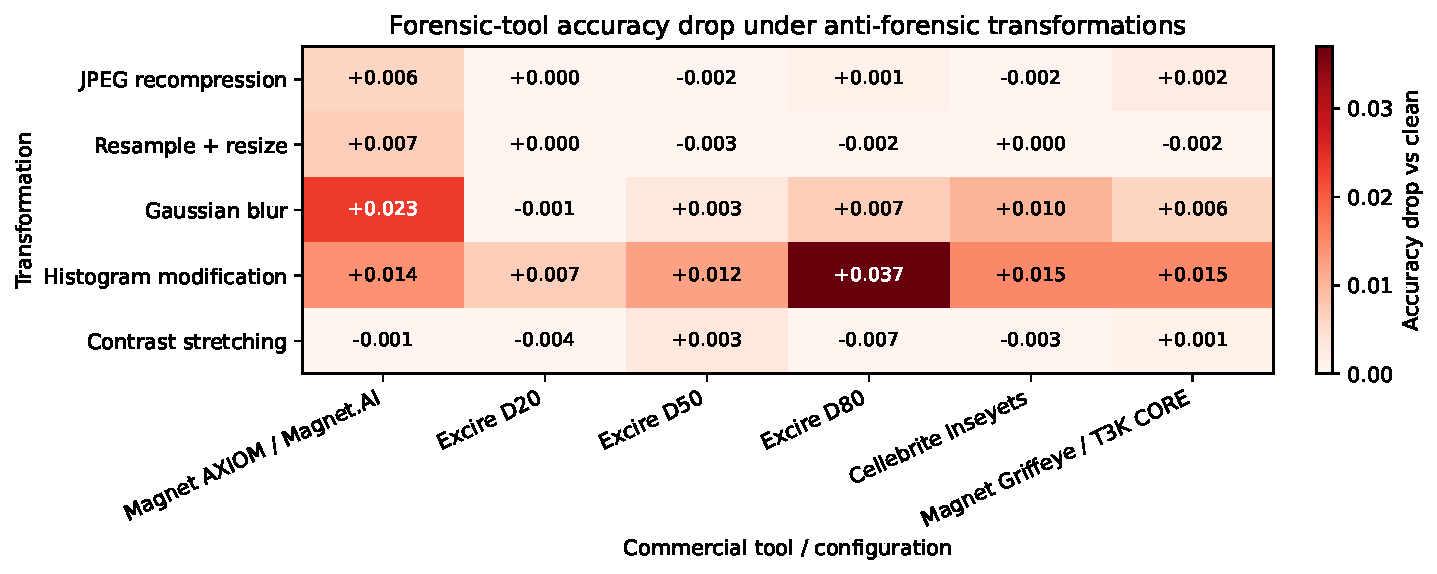
\includegraphics[width=1\textwidth]{images/fig_forensic_tools_anti_forensic_accuracy_drop_heatmap.pdf}
\caption{Accuracy drop of selected black-box software systems under anti-forensic transformations}
\label{fig:results-forensic-tools-antiforensic-drop-heatmap}
\end{figure}

Figure~\ref{fig:results-forensic-tools-antiforensic-drop-heatmap} complements
the tabular interpretation by showing that, for selected software systems,
anti-forensic transformations generally produce limited drops. The most evident
variations are observed for \gls{excirefoto2025} under the \texttt{D80}
configuration with \gls{histogrammodification} and, to a lesser extent, for
\gls{magnetai} under \gls{gaussianblur}. \gls{griffeye}/\gls{t3kcore}
maintains a limited drop, while still exhibiting residual false negatives in
the most critical condition.

The anti-forensic results show generally limited degradation in both proxy
models and selected software systems. This result is important because it
distinguishes the operational effect of plausible transformations from the more
aggressive effect of adversarial perturbations. For EfficientNet-B0, the most
critical condition is \gls{gaussianblur}, which produces 17 induced errors, all
in the \texttt{weapon}\(\rightarrow\)\texttt{non\_weapon} direction. Although
the aggregate drop is limited, this error direction is forensically relevant,
because it corresponds to missed detection of \texttt{weapon} samples.

ResNet18 shows the most marked anti-forensic degradation under
\gls{histogrammodification}, with an accuracy of 0.934 and 39 induced errors.
Unlike EfficientNet-B0, the error pattern is bidirectional: both missed
detections of the \texttt{weapon} class and false \texttt{weapon} flags on
\texttt{non\_weapon} images are present. \gls{clip}, instead, remains
relatively stable with respect to the tested transformations. This confirms
that, in the present protocol, the main criticality of \gls{clip} is not
anti-forensic degradation, but the tendency to map \gls{ood} inputs to the
\texttt{weapon} class.

Selected software systems also show limited aggregate degradation.
\gls{griffeye}/\gls{t3kcore} exhibits the highest aggregate anti-forensic
accuracy, equal to 0.974, followed by \gls{cellebriteinseyets},
\gls{excirefoto2025} under the \texttt{D50} configuration, and \gls{magnetai}.
However, the operational interpretation varies across systems.
\gls{griffeye}/\gls{t3kcore} maintains a very limited \gls{fpr}, but exhibits
residual false negatives under \gls{histogrammodification}.
\gls{cellebriteinseyets} maintains high recall, but with a higher \gls{fpr}
than \gls{griffeye}/\gls{t3kcore}. \gls{magnetai} is more exposed to false
negatives under \gls{gaussianblur}, whereas \gls{excirefoto2025} exhibits a
criticality more attributable to false positive increase under
\gls{histogrammodification}.

\paragraph{Robustness with respect to adversarial perturbations.}

Table~\ref{tab:results-comparative-adversarial} summarizes the adversarial
robustness profile. Unlike anti-forensic transformations, adversarial
perturbations are designed to alter the decision behavior of \gls{ai}-based
systems. For this reason, they produce more heterogeneous and more
model-dependent effects. The results highlight an important distinction among source-model vulnerability
under the defined access assumptions, cross-model transfer across the proxy
architectures, and the operational black-box transfer behavior of the selected
software systems.

\begin{table}[H]
\centering
\caption{Comparison of robustness under adversarial perturbations}
\label{tab:results-comparative-adversarial}
\footnotesize
\renewcommand{\arraystretch}{1.18}
\setlength{\tabcolsep}{3pt}
\begin{tabularx}{\textwidth}{@{}p{2.7cm} p{1.8cm} p{3.1cm} p{2.8cm} X@{}}
\toprule
\textbf{System} &
\textbf{\shortstack{Adversarial\\accuracy/\\drop}} &
\textbf{Most critical condition} &
\textbf{Main error} &
\textbf{Scoped interpretation} \\
\midrule

EfficientNet-B0 &
0.695 / 0.283 &
\gls{sigmazero}; acc. 0.015; drop 0.963 &
963 induced errors; 489 W$\rightarrow$NW and 474 NW$\rightarrow$W &
Most marked proxy vulnerability in the white-box scenario; high clean accuracy
does not guarantee adversarial robustness. \\

ResNet18 &
0.955 / 0.009 &
\gls{fgsm}; acc. 0.918; drop 0.046 &
47 induced errors; 27 W$\rightarrow$NW and 20 NW$\rightarrow$W &
Limited aggregate degradation; the model-dependent results reflect cross-model
transfer, with residual degradation under \gls{fgsm}. The evaluation does not
represent a direct white-box assessment of ResNet18. \\

\gls{clip} &
0.927 / 0.000 &
\gls{fgsm}; acc. 0.914; drop 0.013 &
23 induced errors; 8 W$\rightarrow$NW and 15 NW$\rightarrow$W &
Limited aggregate degradation; the model-dependent results reflect cross-model
transfer and do not demonstrate direct adversarial robustness. The distinct \gls{ood}
assignment behavior must be considered separately. \\

\gls{magnetaxiomtool}/\gls{magnetai} &
0.923 / 0.027 &
\gls{fgsm}; acc. 0.867; \acrshort{fnr} 0.192 &
96 \acrshort{fn} &
Aggregate accuracy decreases by 0.027, while \gls{fgsm} substantially increases
false negatives on the \texttt{weapon} class. \\

\gls{griffeye}/\gls{t3kcore} &
0.969 / 0.009 &
\gls{sigmazero}; acc. 0.959; \acrshort{fnr} 0.074 &
37 \acrshort{fn} &
Highest aggregate normalized accuracy among the selected black-box
configurations under adversarial artifacts; the low \gls{fpr} also reflects the
conservative mapping, while residual degradation remains. \\

\gls{excirefoto2025} \texttt{D50} &
0.904 / 0.040 &
\gls{sigmazero}; acc. 0.742; \acrshort{fpr} 0.442 &
221 \acrshort{fp} &
The principal effect is an increase in firearm-prompt retrievals for
\texttt{non\_weapon} samples rather than systematic concealment of
\texttt{weapon} images. \\

\gls{cellebriteinseyets} &
0.955 / 0.009 &
\gls{fgsm}; acc. 0.918; \acrshort{fnr} 0.106 &
53 \acrshort{fn} &
Limited aggregate degradation under the transferred adversarial artifacts,
with an increase in false negatives especially under \gls{fgsm}. \\

\bottomrule
\end{tabularx}

\vspace{0.4em}
\footnotesize
\textit{Note.} For the proxy models, aggregate values are computed across the
five adversarial perturbations considered. For selected software systems,
values derive from the normalized outputs on the forensic evaluation bundle.
The drop is defined in Section~\ref{sec:results-scope}. W$\rightarrow$NW
indicates transitions from \texttt{weapon} to \texttt{non\_weapon}; \acrshort{fn}
indicates false negatives; \acrshort{fnr} indicates false negative rate; \acrshort{fpr} indicates
false positive rate.
\end{table}

\begin{figure}[H]
\centering
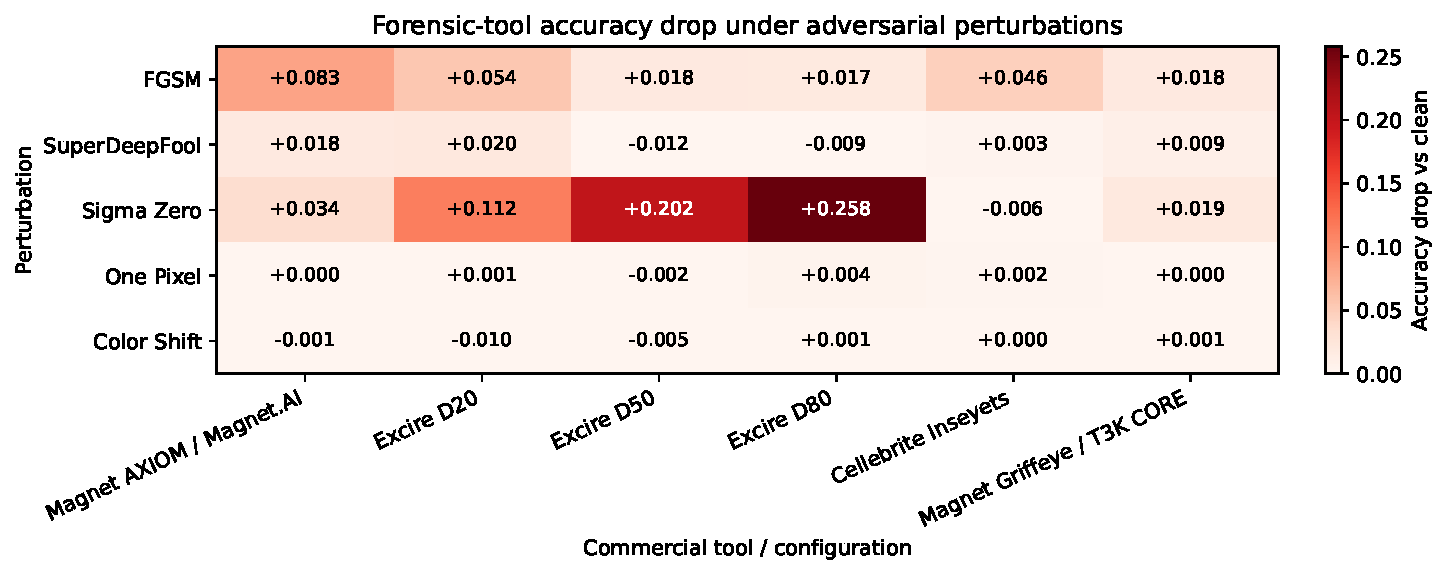
\includegraphics[width=1\textwidth]{images/fig_forensic_tools_adversarial_accuracy_drop_heatmap.pdf}
\caption{Accuracy drop of selected black-box software systems under adversarial perturbations}
\label{fig:results-forensic-tools-adversarial-drop-heatmap}
\end{figure}

Figure~\ref{fig:results-forensic-tools-adversarial-drop-heatmap} shows that the
response of selected software systems to adversarial perturbations is strongly
dependent on the system and configuration. \gls{excirefoto2025} is particularly
sensitive to \gls{sigmazero} under the \texttt{D50} and \texttt{D80}
configurations, whereas \gls{cellebriteinseyets} and
\gls{griffeye}/\gls{t3kcore} show more limited aggregate drops. This result
reinforces the interpretation that the operational robustness of selected
black-box software systems is not uniform, but depends on the type of
observable output, the adopted mapping, and the system configuration.

The adversarial comparison shows that the most severe degradation occurs at the
proxy level, particularly for EfficientNet-B0 under \gls{sigmazero}. The model
moves from a clean accuracy of 0.978 to an accuracy of 0.015, with 963 induced
errors. This result shows, in the considered protocol, that a model may be very
accurate under nominal conditions and, at the same time, extremely fragile with
respect to optimized adversarial perturbations. \gls{fgsm} also produces
significant degradation for EfficientNet-B0, with an accuracy of 0.575 and a
drop of 0.403. The observed vulnerability is therefore not limited to a single
adversarial condition.

ResNet18 and \gls{clip} show a more stable profile in the present experimental
setting. ResNet18 is most affected by \gls{fgsm}, but the drop remains much
lower than that observed for EfficientNet-B0. \gls{clip} is even less degraded
by the tested perturbations. However, this result must be interpreted with caution: the model-dependent
attacks were generated against EfficientNet-B0 rather than against \gls{clip}.
The observed behavior of \gls{clip} therefore represents cross-model transfer
under the evaluated conditions, not direct source-model robustness.
Furthermore, \gls{clip} exhibits a distinct criticality on \gls{ood} inputs.
The observed adversarial stability must consequently not be generalized beyond
the evaluated threat model.

Selected software systems show a different pattern. \gls{magnetai} does not
reproduce the catastrophic degradation observed for EfficientNet-B0 under
\gls{sigmazero}, but is substantially affected by \gls{fgsm}, with a
\gls{fnr} of 0.192. From a forensic perspective, this is a critical error,
because the missed detection of \texttt{weapon} images may lead to the
deprioritization of relevant material.

\gls{excirefoto2025} under the \texttt{D50} configuration instead reacts
differently: \gls{sigmazero} primarily produces an increase in the false
positive rate, equal to 0.442, generating semantic over-triggering rather than
systematic concealment of the \texttt{weapon} class. \gls{cellebriteinseyets}
shows high recall and limited degradation, but maintains a higher false
positive rate than \gls{griffeye}/\gls{t3kcore}. Under the adopted conservative
mapping, \gls{griffeye}/\gls{t3kcore} exhibits the highest aggregate black-box
accuracy and the lowest false positive rate, while still retaining residual
false negatives on the \texttt{weapon} class.

Overall, the comparison among selected software systems does not identify a
single preferable system across all operational criteria, but highlights
different operating profiles. \gls{griffeye}/\gls{t3kcore} exhibits the most
selective profile and the lowest operational noise in terms of false positives;
\gls{cellebriteinseyets} maintains slightly higher recall on the
\texttt{weapon} class; \gls{excirefoto2025} shows behavior strongly dependent
on the retrieval threshold; and \gls{magnetai} exhibits a more conservative
profile but with a higher false negative rate. This heterogeneity shows that
the observed operating profiles of the selected black-box software systems
depend on the software configuration, observable
output, normalization mapping, and role assigned to the analyst in the
workflow.

\paragraph{Threshold sensitivity and black-box interpretation.}

The results of \gls{excirefoto2025} require a separate interpretation, because
the system was evaluated as a semantic retrieval engine and not as a native
forensic classifier. The \texttt{Distance limit} parameter defines the
operational restrictiveness of semantic retrieval. The \texttt{D20}
configuration is restrictive: it reduces false positives and weapon flags on
\gls{ood} inputs, but increases the risk of missed detection of
\texttt{weapon} images. The \texttt{D80} configuration is permissive: it
maximizes recall, but increases false positives and the assignment of
non-relevant or perturbed images to the semantic query related to weapons. The
\texttt{D50} configuration was used as the main comparison point because it
represents an intermediate profile.

This threshold dependence is particularly evident under \gls{sigmazero}. Under
the \texttt{D20} configuration, \gls{excirefoto2025} achieves an accuracy of
0.815, an \acrshort{fnr} of 0.180, and an \acrshort{fpr} of 0.190. Under the \texttt{D50}
configuration, accuracy decreases to 0.742, while \acrshort{fnr} improves to 0.074 and
\acrshort{fpr} increases to 0.442. Under the \texttt{D80} configuration, recall improves
further, but \acrshort{fpr} rises to 0.662. The same software system can therefore support
different forensic priorities depending on the selected operating point:
\texttt{D20} prioritizes the containment of operational noise,
\texttt{D80} prioritizes recall, and \texttt{D50} represents an intermediate
trade-off between false negatives and false positives.

The black-box nature of selected software systems also limits the types of
conclusions that can be drawn. Unlike the proxy models, these systems do not
expose decision boundaries, calibrated scores, architectures, training data, or
internal thresholding logic. Their outputs can therefore be evaluated only at
the operational level, through observable categories, exported tags, retrieval
results, semantic bookmarks, matching rate, non-mappable outputs, false
negatives, false positives, and behavior on \gls{ood} inputs. This limitation
does not represent a weakness of the evaluation protocol; on the contrary, it
reflects the operational condition in which forensic analysts interact with
selected black-box \gls{ai}-assisted software systems.


Figure~\ref{fig:results-operational-risk-summary} summarizes the main
quantitative operating dimensions discussed in the comparative analysis. The
figure
does not encode interpretability as a numerical score, since the distinction
between inspectable proxy models and black-box software systems represents a
methodological condition rather than an experimentally measured variable.

\begin{figure}[H]
    \centering
    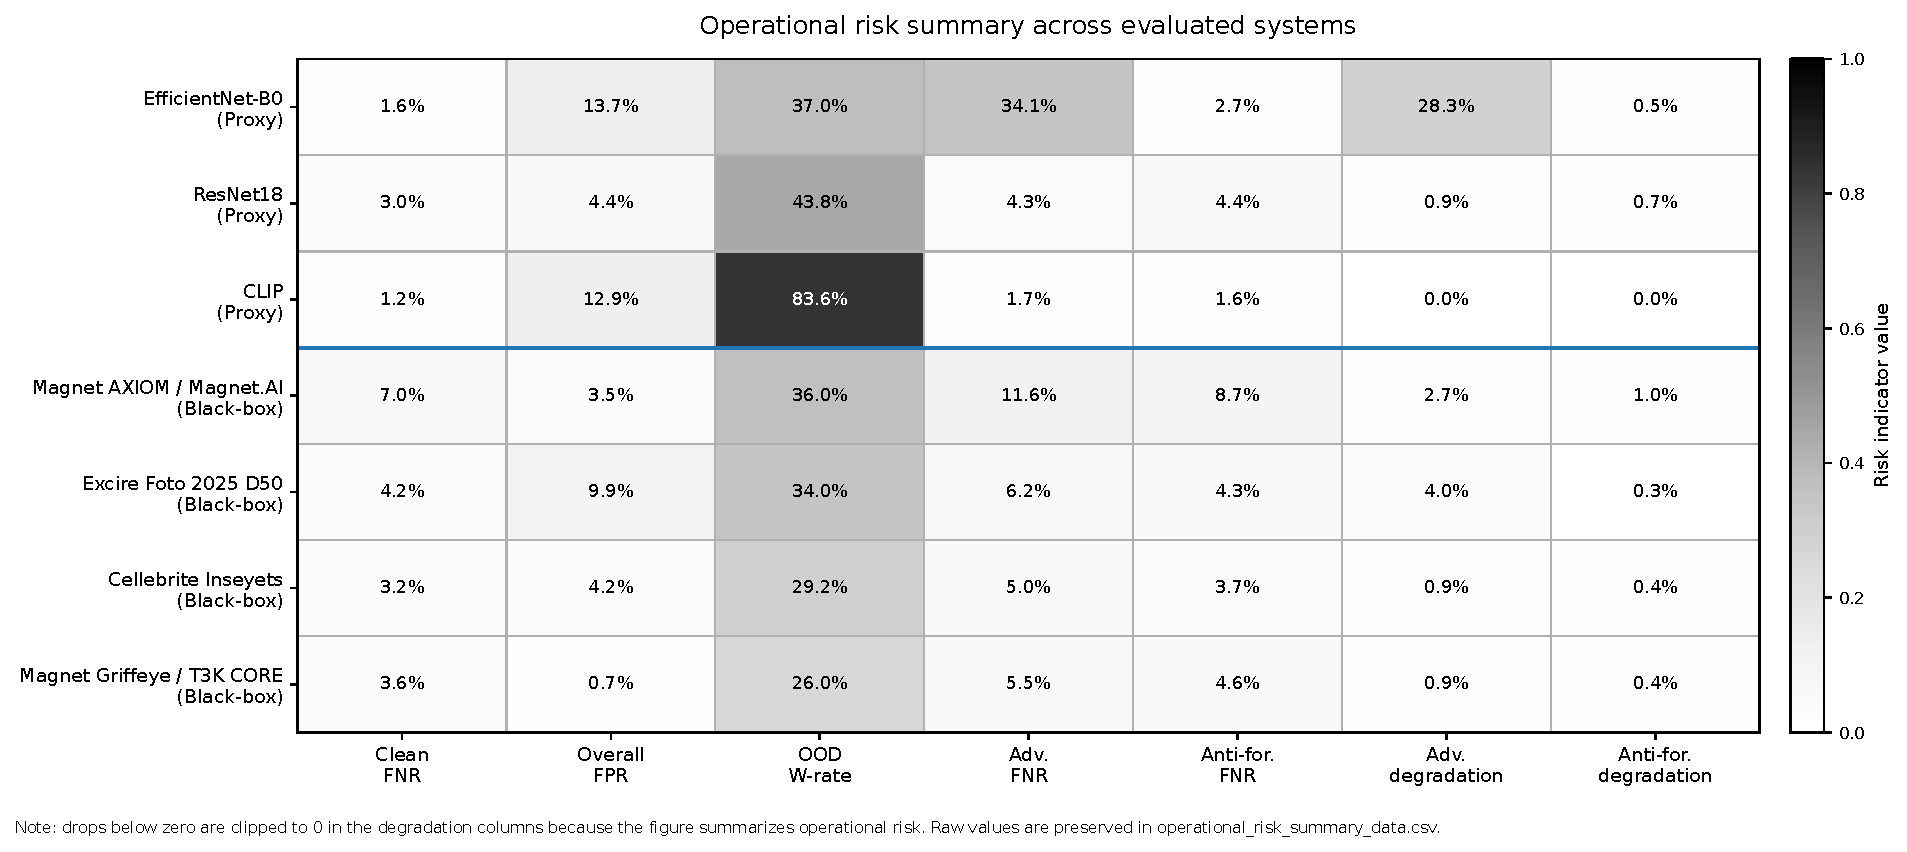
\includegraphics[width=\textwidth]{images/fig_results_operational_risk_summary.pdf}
   \caption[Operational behavior summary across evaluated systems]{Operational
behavior indicators across proxy models and selected black-box software
configurations}
\label{fig:results-operational-risk-summary}

\end{figure}


\begin{flushleft}
\footnotesize
\textit{Note.} Clean \acrshort{fnr} is computed on the unperturbed binary subset. Bundle
\acrshort{fpr} is computed on the complete binary bundle, including clean,
adversarial, and anti-forensic samples and excluding \gls{ood} samples.
Adversarial \acrshort{fnr} and anti-forensic \acrshort{fnr} are aggregated across the corresponding
perturbation families. \acrshort{ood} W-rate reports the proportion of \gls{ood} samples
mapped to the operational \texttt{weapon} class. Accuracy drops are computed
with respect to the clean baseline; slightly negative values are interpreted as
negligible distribution-specific oscillations.
\end{flushleft}

\paragraph{Overall operational interpretation.}

The comparative analysis confirms that robustness in \gls{ai}-assisted forensic
image triage is a multidimensional property. Clean accuracy measures nominal
performance, but it does not capture \gls{ood} weapon assignment behavior,
sensitivity to
perturbations, false negative rates, semantic over-triggering, or the effect of
thresholds in black-box systems. In \gls{df} workflows, these dimensions are at
least as relevant as aggregate accuracy, because they influence analyst
attention, content prioritization, and the manual review strategy.

Three main findings emerge. First, proxy models are useful because they make
controlled degradation patterns observable and allow confidence shift, induced
errors, and error direction to be measured. However, their behavior cannot be
automatically transferred to selected software systems because their internal
mechanisms for classification, tagging, retrieval, and semantic-bookmark
generation are inaccessible. Second, selected software systems show differentiated operating profiles:
some privilege recall, others reduce false positives, and others depend strongly
on the retrieval configuration or adopted semantic mapping. Third, \gls{ood}
behavior remains a distinct evaluation dimension because weapon-oriented outputs
on this branch may increase analyst workload or affect prioritization even
though they are not supervised binary errors.

Overall, the results support a cautious interpretation of \gls{ai}-based
automation in forensic contexts. The evaluated systems can provide useful
support for triage, prioritization, and large-scale review of multimedia
content. However, their outputs must not be treated as conclusive evidence or
as substitutes for expert validation. In particular, missed detections of
\texttt{weapon} images, high-confidence \gls{ood} assignments, and threshold-dependent
errors must be explicitly documented when \gls{ai}-assisted software systems
are used in forensic workflows. The \gls{fairlab} protocol responds to this
need by combining frozen datasets, traceable manifests, hash-based
reproducibility, controlled perturbation families, black-box output
normalization, and manual auditability of the final interpretation.

% ─────────────────────────────────────────────────────────────────────────────
\section{Explainability Analysis and Representative Failure Cases}
\label{sec:results-explainability}
% ─────────────────────────────────────────────────────────────────────────────

The \gls{xai} analysis was used as a qualitative and diagnostic tool to connect
the aggregate metrics discussed in the previous sections to a restricted set of
representative cases. It does not constitute a primary robustness metric and
does not replace quantitative measures of accuracy, confidence, false positives,
and false negatives. Its role is instead to support the operational
interpretation of selected behaviors observed in the proxy model, by
showing the spatial distribution of attribution magnitude for the selected
model output in specific success or failure scenarios.

The attribution maps were generated using \gls{ig} applied to the white-box
EfficientNet-B0 proxy model, with the model-predicted class as the attribution
target, indicated in the experimental files as \texttt{predicted\_label}.
This choice associates each visualization with the output actually produced
by the model rather than with the reference operational assignment. In erroneous
cases, the map therefore represents attribution magnitude for the incorrect
predicted class.

The generated maps must not be interpreted as direct explanations of the
behavior of \gls{magnetaxiomtool}/\gls{magnetai},
\gls{excirefoto2025}, \gls{cellebriteinseyets}, or
\gls{griffeye}/\gls{t3kcore}, which remain black-box systems in the context of
this evaluation. Rather, they provide a controlled diagnostic reference, limited
to the white-box proxy model, and support discussion of selected proxy-model
behaviors in a \gls{df}
\textit{human-in-the-loop} context.

The \gls{xai} figures reported in this section follow the generation and
selection procedure documented in
Section~\ref{subsec:implementation-explainability}: input image, \gls{ig}
heatmap, attribution overlay on the original image, and mask of the locations
with the largest attribution magnitudes. The attribution mask must not be interpreted as a
semantic segmentation,
object-level annotation, or causal explanation. It visualizes the locations with
the largest absolute attribution magnitudes under the adopted baseline and
target. Similarly, the reported score is the proxy model's maximum
predicted-class probability and is not treated as calibrated.

As documented in Section~\ref{subsec:implementation-explainability}, the
retained historical figures were generated using 32 integration steps and are
interpreted exclusively as qualitative diagnostic visualizations. No strict
numerical convergence claim is made for these assets.

Table~\ref{tab:results-xai-cases} summarizes the five cases selected for the
qualitative analysis. The selection covers one correct case on a clean input,
one false negative on a clean input, one \gls{ood} case assigned to
\texttt{weapon}, one false negative produced by an anti-forensic transformation,
and one high-confidence adversarial false positive.

\begin{table}[htbp]
\centering
\small
\renewcommand{\arraystretch}{1.15}
\setlength{\tabcolsep}{4pt}
\caption{Representative cases selected for the qualitative analysis of EfficientNet-B0 using \gls{ig}}
\label{tab:results-xai-cases}
\begin{tabularx}{\textwidth}{@{}p{0.17\textwidth} p{0.15\textwidth} p{0.13\textwidth} p{0.13\textwidth} X@{}}
\toprule
\textbf{Identifier} &
\textbf{Scenario} &
\textbf{Reference state} &
\textbf{Prediction} &
\textbf{Operational role} \\
\midrule

\texttt{xai\_case\_0001} &
\texttt{clean} &
\texttt{weapon} &
\texttt{weapon} &
Correct case on a clean input, used as a reference for observing coherent
attribution behavior. \\

\texttt{xai\_case\_0006} &
\texttt{clean} &
\texttt{weapon} &
\texttt{non\_weapon} &
False negative on a clean input, representative of missed detection in the
absence of perturbations. \\

\texttt{xai\_case\_0009} &
\texttt{ood} &
\texttt{ood} &
\texttt{weapon} &
\gls{ood} input assigned to \texttt{weapon}, representing a closed-set
assignment on the separate evaluation branch. \\

\texttt{xai\_case\_0010} &
\gls{histogrammodification} &
\texttt{weapon} &
\texttt{non\_weapon} &
Anti-forensic false negative, representative of the effects of low-level visual
manipulations. \\

\texttt{xai\_case\_0015} &
\gls{sigmazero} &
\texttt{non\_weapon} &
\texttt{weapon} &
High-score adversarial false positive, representative of the unreliability of
the maximum predicted-class probability as a stand-alone reliability indicator. \\

\bottomrule
\end{tabularx}
\vspace{0.4em}
\footnotesize
\textit{Note.} For \texttt{xai\_case\_0009}, \texttt{ood} denotes the separate
\gls{ood} evaluation branch and not a third supervised class.
\end{table}

\XAIcaseFigureMaskGrid
{fig:xai-case1-clean-correct}
{Correct case on a clean input \texttt{xai\_case\_0001}. The EfficientNet-B0
proxy model correctly classifies a \texttt{clean} image with reference
operational assignment \texttt{weapon} as \texttt{weapon}}
{images/fig_xai_case1_clean_correct_input.png}
{images/fig_xai_case1_clean_correct_heatmap.png}
{images/fig_xai_case1_clean_correct_overlay.png}
{images/fig_xai_case1_clean_correct_top10_mask.png}
{\textbf{scenario}: \texttt{clean};
\textbf{reference state}: \texttt{weapon};
\textbf{prediction}: \texttt{weapon};
\textbf{confidence}: 1.000}

The first case, shown in Figure~\ref{fig:xai-case1-clean-correct}, provides a
qualitative reference in which the model prediction is consistent with the
reference operational assignment. The image belongs to the \texttt{clean}
scenario, its reference operational
assignment is \texttt{weapon}, and EfficientNet-B0 also predicts
\texttt{weapon}, with a maximum predicted-class probability of 1.000. In this
case, the \gls{ig} map supports inspection of whether larger attribution
magnitudes overlap the visually salient object region or are concentrated on
background and contextual elements. This example does not, by
itself, demonstrate the general reliability of the model, but serves as a
reference case against which the subsequent failures can be compared.

\XAIcaseFigureMaskGrid
{fig:xai-case2-clean-false-negative}
{False negative on a clean input \texttt{xai\_case\_0006}. A \texttt{clean}
image with reference operational assignment \texttt{weapon} is classified as
\texttt{non\_weapon}}
{images/fig_xai_case2_clean_false_negative_input.png}
{images/fig_xai_case2_clean_false_negative_heatmap.png}
{images/fig_xai_case2_clean_false_negative_overlay.png}
{images/fig_xai_case2_clean_false_negative_top10_mask.png}
{\textbf{scenario}: \texttt{clean};
\textbf{reference state}: \texttt{weapon};
\textbf{prediction}: \texttt{non\_weapon};
\textbf{confidence}: 0.692}

The second case, reported in
Figure~\ref{fig:xai-case2-clean-false-negative}, is relevant because the error
occurs on a clean input, without adversarial perturbations or anti-forensic
transformations. The image has the reference operational assignment
\texttt{weapon}, but
EfficientNet-B0 classifies it as \texttt{non\_weapon} with a maximum
predicted-class probability of 0.692.
In a \gls{df} workflow, this type of error may have a direct operational
consequence because a false negative may prevent a potentially relevant image
from being prioritized during automated triage.

The corresponding \gls{ig} map makes it possible to inspect whether the
largest attribution magnitudes are localized on the object region or distributed
across contextual elements. This case shows that good aggregate performance on \texttt{clean} data does not eliminate
the need for human assessment, especially when the automatic result is used to
filter or rank large volumes of images in an investigative context.

\XAIcaseFigureMaskGrid
{fig:xai-case3-ood-as-weapon}
{\gls{ood} case \texttt{xai\_case\_0009}. An \gls{ood} input is
assigned to \texttt{weapon} with a high maximum predicted-class probability}
{images/fig_xai_case3_ood_as_weapon_input.png}
{images/fig_xai_case3_ood_as_weapon_heatmap.png}
{images/fig_xai_case3_ood_as_weapon_overlay.png}
{images/fig_xai_case3_ood_as_weapon_top10_mask.png}
{\textbf{scenario}: \texttt{ood};
\textbf{reference state}: \texttt{ood};
\textbf{prediction}: \texttt{weapon};
\textbf{confidence}: 0.999}

The third case, shown in Figure~\ref{fig:xai-case3-ood-as-weapon}, differs from
an ordinary false positive because the sample belongs to the separate \gls{ood}
evaluation branch and has no binary reference assignment. EfficientNet-B0 maps
it to \texttt{weapon} with a maximum predicted-class probability of 0.999.
The \gls{ood} branch includes borderline, distributionally atypical, degraded,
synthetic, or semantically out-of-task cases rather than a homogeneous class of
realistic negatives.

The \gls{ig} visualization shows whether larger attribution magnitudes for
the predicted \texttt{weapon} output are localized or distributed across the
input. It does not establish that the highlighted regions correspond to
firearm-specific features. From a methodological perspective, this case
supports the choice to preserve \texttt{ood} as a separate dataset and evaluation branch, rather than treating
it as a third supervised class or merging all inputs outside the
\texttt{weapon} class into the \texttt{non\_weapon} class.

\XAIcaseFigureMaskGrid
{fig:xai-case4-antiforensic-failure}
{Anti-forensic false negative \texttt{xai\_case\_0010}. A \texttt{weapon} image
subjected to \gls{histogrammodification} is classified as
\texttt{non\_weapon}}
{images/fig_xai_case4_antiforensic_failure_input.png}
{images/fig_xai_case4_antiforensic_failure_heatmap.png}
{images/fig_xai_case4_antiforensic_failure_overlay.png}
{images/fig_xai_case4_antiforensic_failure_top10_mask.png}
{\textbf{scenario}: \gls{histogrammodification};
\textbf{reference state}: \texttt{weapon};
\textbf{prediction}: \texttt{non\_weapon};
\textbf{confidence}: 0.852}

The fourth case, reported in
Figure~\ref{fig:xai-case4-antiforensic-failure}, concerns an anti-forensic
transformation based on \gls{histogrammodification}. The reference operational
assignment remains \texttt{weapon}, but the model predicts
\texttt{non\_weapon} with a maximum predicted-class probability of
0.852. The case is relevant because the transformation is not an adversarial
perturbation optimized against a differentiable model. It is instead a
low-level visual manipulation that affects tonal distribution, contrast, and
the local representation of image structures.

The \gls{ig} map enables comparison of the attribution distribution observed
for this transformed input, but it does not isolate the causal mechanism through
which histogram modification changed the prediction. From an operational
perspective, this failure suggests that transformations that may remain visually recognizable to human analysts can
nevertheless compromise automated classification. In a forensic pipeline, this
reinforces the need not to treat the classifier output as autonomous evidence,
but as support to be critically verified.

\XAIcaseFigureMaskGrid
{fig:xai-case5-adversarial-high-confidence-failure}
{High-confidence adversarial false positive \texttt{xai\_case\_0015}. A
\texttt{non\_weapon} image perturbed using \gls{sigmazero} is classified as
\texttt{weapon}}
{images/fig_xai_case5_adversarial_high_conf_failure_input.png}
{images/fig_xai_case5_adversarial_high_conf_failure_heatmap.png}
{images/fig_xai_case5_adversarial_high_conf_failure_overlay.png}
{images/fig_xai_case5_adversarial_high_conf_failure_top10_mask.png}
{\textbf{scenario}: \gls{sigmazero};
\textbf{reference state}: \texttt{non\_weapon};
\textbf{prediction}: \texttt{weapon};
\textbf{confidence}: 1.000}

The fifth case, shown in
Figure~\ref{fig:xai-case5-adversarial-high-confidence-failure}, represents a
high-confidence adversarial false positive. The image has the reference
operational assignment \texttt{non\_weapon}, but, after the \gls{sigmazero} perturbation, it is
classified as \texttt{weapon} with a maximum predicted-class probability of
1.000. For the purposes of this thesis, this case is particularly significant because it separates two
concepts that may be incorrectly conflated in an operational workflow: the
maximum predicted-class probability and the forensic reliability of the
prediction.

The \gls{ig} visualization provides a diagnostic representation of
attribution magnitude for the incorrect predicted class, but it must not be
interpreted as a complete explanation of the attack mechanism. Its value lies
in making a high-score failure directly observable and showing that a maximum
predicted-class probability of 1.000 does not establish operational
reliability. In an investigative context, this
result supports the need to maintain the \textit{human-in-the-loop} paradigm,
especially when \gls{ai}-based systems are used to prioritize sensitive or
potentially relevant content.

Overall, the five selected cases show that \gls{xai} analysis can provide a
useful interpretive contribution, provided that its role remains properly
delimited. The correct case on a clean input serves as a qualitative reference
for coherent attribution behavior; the false negative on a clean input shows
that missed detection can occur even in the absence of manipulation; the
\gls{ood} case documents a closed-set \texttt{weapon} assignment on the
separate evaluation branch; the anti-forensic case shows that low-level visual
transformations can alter the automatic decision; and the high-confidence
adversarial case shows that confidence cannot be assumed as a sufficient
indicator of operational reliability.

For these reasons, \gls{xai} analysis is considered in this thesis as support
for understanding representative cases and not as autonomous evidence of system
robustness. It makes selected behaviors of the EfficientNet-B0 proxy model more
transparent, but it does not automatically extend its conclusions to selected
black-box software systems. In a \gls{df} pipeline, visualizations based on
\gls{ig} must therefore be interpreted as instruments supporting review,
evaluation, and critical discussion of the results, while preserving the central
role of the human analyst in the final assessment.


% ─────────────────────────────────────────────────────────────────────────────
\section{Operational Interpretation and Experimental Limitations}
\label{sec:results-limitations}
% ─────────────────────────────────────────────────────────────────────────────

The results show that the operational robustness of \gls{ai}-based systems for
forensic image classification and triage cannot be inferred from clean accuracy
alone. Interpretation must jointly consider the direction of the errors,
behavior on \gls{ood} inputs, degradation under manipulated conditions,
threshold- or mapping-dependent trade-offs, and the extent to which the output
remains auditable and subject to human verification.

False negatives and false positives have different operational consequences. A
false negative on the \texttt{weapon} class may prevent potentially relevant
content from being prioritized for review. A false positive may instead
increase analyst workload and dilute
prioritization. A \texttt{weapon} assignment on an \gls{ood} input is not a
binary error, but may produce similar workload or prioritization effects.
Aggregate accuracy therefore provides only a partial description of the
observed operating profile.

The parallel comparison also demonstrates that nominally strong systems may
fail under different conditions. EfficientNet-B0 achieves the highest clean
accuracy among the proxy models but undergoes severe white-box degradation
under \gls{sigmazero} and substantial degradation under \gls{fgsm}. The
selected black-box software systems do not exhibit the same collapse on those
artifacts, but their observable outputs reveal other limitations, including
missed detections, false-positive workload, configuration sensitivity, and
non-zero \gls{ood} weapon-flag rates. These differences reinforce the need to
evaluate systems through multiple operational conditions rather than a single
clean benchmark.

Several limitations define the scope of the findings.

\begin{itemize}
    \item The frozen dataset contains 1\,500 manually selected images and does
    not represent the full diversity of firearm-related, non-firearm, and
    \gls{ood} imagery encountered in operational investigations.
    Selection was performed by a single reviewer; no inter-rater agreement was
    measured.

    \item The source distribution is not uniform. In particular, the
    \texttt{non\_weapon} branch is predominantly derived from
    \texttt{05\_deepweb}. Source-specific regularities may therefore influence
    some observed results despite the source-aware fold construction.

    \item The four model-dependent adversarial attacks were generated against
    fold-aware EfficientNet-B0 checkpoints. The resulting cross-model and
    black-box analyses measure transfer behavior of those artifacts, not a
    complete attack space optimized independently against every evaluated
    system.

    \item The adversarial and anti-forensic suites are finite and use one frozen
    parameterization per condition. Different budgets, severities, image
    encodings, attack implementations, or transformation combinations may
    produce different robustness profiles.

    \item The proxy architectures are transparent experimental references and
    must not be interpreted as reconstructions of the internal models used
    by the selected software systems.

    \item Black-box results depend on the evaluated software versions, enabled
    functions, export formats, and explicit normalization rules. The conservative
    firearm-bookmark mapping adopted for \gls{griffeye}/\gls{t3kcore} and the
    distance setting adopted for \gls{excirefoto2025} directly affect the
    observed balance between missed detections and false-positive workload.

    \item Proxy-model \gls{ood} rates aggregate five predictions per image,
    whereas black-box rates use one normalized decision per image. The resulting
    proportions support parallel descriptive comparison but do not constitute
    identical statistical observations.

    \item The retained \gls{xai} analysis is limited to five representative
    EfficientNet-B0 cases. The historical assets were generated with 32
    integration steps and are used only for qualitative interpretation; no
    strict convergence claim is made, and the findings cannot be extended to
    the selected black-box software systems.

    \item The embedded-metadata audit identified a small residual information
    channel in the blind bundle. The leave-out analysis indicates limited
    quantitative influence on the reported aggregate metrics. However, the frozen
    protocol did not include a separate metadata-neutralized comparison bundle, and
    the corresponding analysis therefore remains limited to the
    metadata-preserving bundle used in the experiment.
\end{itemize}

These limitations delimit the conditions under which the experimental
conclusions are supported. The chapter therefore
provides a protocol-specific assessment of operational robustness rather than
a software-system certification, universal robustness ranking, or
evidentiary validation of automated outputs.

The practical implication is that automated image-analysis systems should be
used as traceable triage support within a \textit{human-in-the-loop} workflow.
Their outputs should remain associated with the source item, system version,
configuration, observable mapping, and relevant uncertainty or limitation. In
particular, missed detections, configuration-dependent behavior, high-confidence
failures, and \gls{ood} assignments must remain visible to the analyst rather
than being hidden behind a single aggregate score.
